\documentclass[Master]{subfiles}
\begin{document}
\section{Results}
We begin by verifying the analytical results for the Hamiltonian with and without vortices present. We observe the spectrum and the critical points and how pots in the chemical potential and a phase winding around the pots change the spectrum. We then analyse the operators of the approximately zero-energy mode. Then the exchange in the adiabatic limit is explored by analysing the instantaneous eigenstates. Finally, we explore the finite time exchange of two and four vortices for different vortex radii and distances.
\subsection{Single Phase}
To verify the analytical observations made in \secref{sec:HamilPhases} we diagonalise the Hamiltonian with periodic boundary conditions and a constant chemical potential. So the case with no vortives present.
\begin{figure}[H]
    \centering
    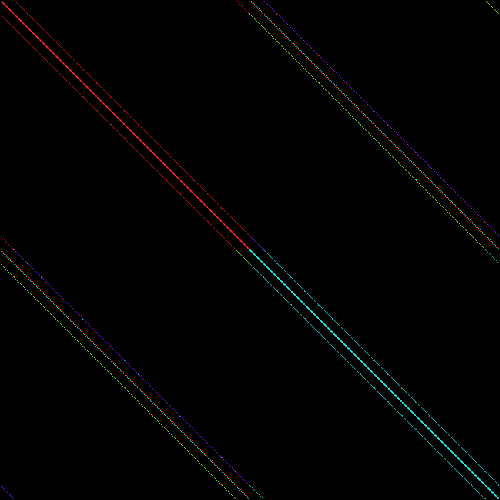
\includegraphics[width=0.4\textwidth]{imgs/Matrix_Periodic_nP_nV.png}
    \caption{$M$ Matrix of the BdG Hamiltonian with periodic boundary conditions. constant Chemical potential $\mu = -2$, tunneling energy $t=\frac{1}{4}$, and Order parameter $|\Delta| = 1,$  on a $35 \times 35 Grid$}
    \label{fig:PeriodicBoundMatrix}
\end{figure}
\begin{figure}[H]
    \centering
    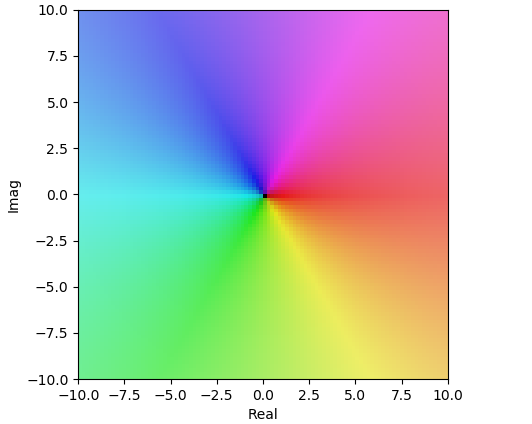
\includegraphics[width=0.3\linewidth]{imgs/Color Wheel.png}
    \caption{Map of $\mathbb{C}$ to colours representing phase and absolute value}
    \label{fig:ComplexColorMap}
\end{figure}
\figref{fig:PeriodicBoundMatrix} shows the spectrum of the matrix. The colours in this figure represents complex numbers as in \figref{fig:ComplexColorMap}. We can observe the block matrix structure. 
$$
M = \left(
\begin{array}{c|c}
A & B \\
\hline
- B^* & -A^*
\end{array}
\right)
$$
The diagonal on the $A$ matrices corresponds to the chemical potential $\mu$. The first off-diagonals correspond to the hopping term $t$ in $x$ direction and the further off-diagonals to the hopping term in the $y$ direction. The $B$ matrices have zero on the diagonals. The same off-diagonals as in the $A$ matrix occur, but with a phase. Here these correspond to the cross Order Parameter term $\Delta$. These have complex-phase. The furthest off-diagonals of the $A$ and $B$ matrices, extending the off-diagonals into the next matrix block are the periodic boundary terms. We plot the eigenvalues for fixed $t=\frac{1}{4}, \Delta = 1$ along the $\mu$ axis to reveal the spectrum of this system \figref{fig:Spectrum_nP_Periodic}.
\begin{figure}[H]
    \centering
    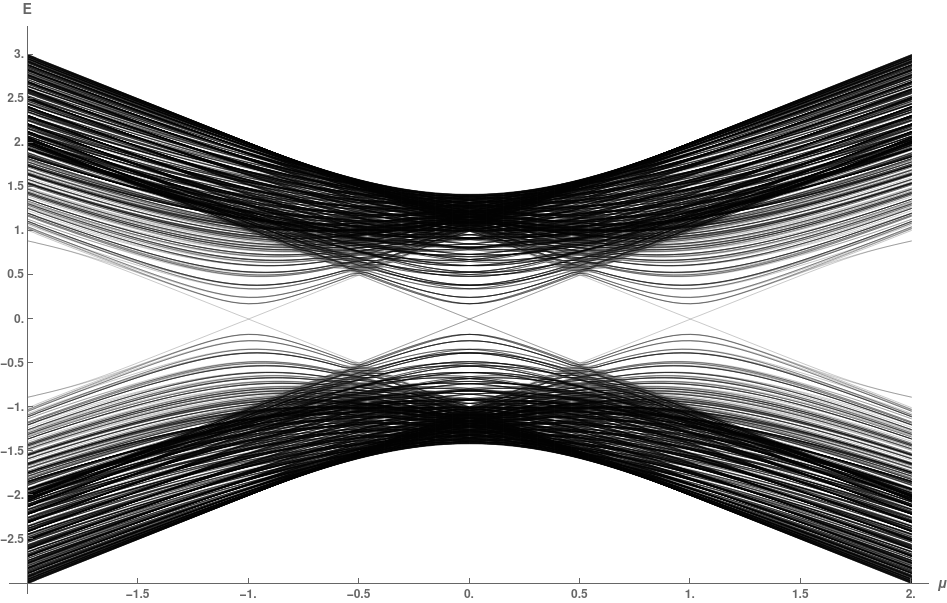
\includegraphics[width=\linewidth]{imgs/Spectrum_nP_Periodic.png}
    \caption{Spectrum for the Hamiltonian with periodic boundary conditions. constant Chemical potential $\mu = -2$, tunneling energy $t=\frac{1}{4}$, and Order parameter $|\Delta| = 1,$  on a $35 \times 35 Grid$.}
    \label{fig:Spectrum_nP_Periodic}
\end{figure}

We see the roots at values for the chemical potential of $\mu = {-4t, 0, 4t}$ exactly where predicted in \secref{sec:HamilPhases}
When we remove the periodic boundary conditions, we observe states equidistantly spaced around zero, as we show in \figref{fig:Spectrum_nP_nPeriodic}.
\begin{figure}[H]
    \centering
    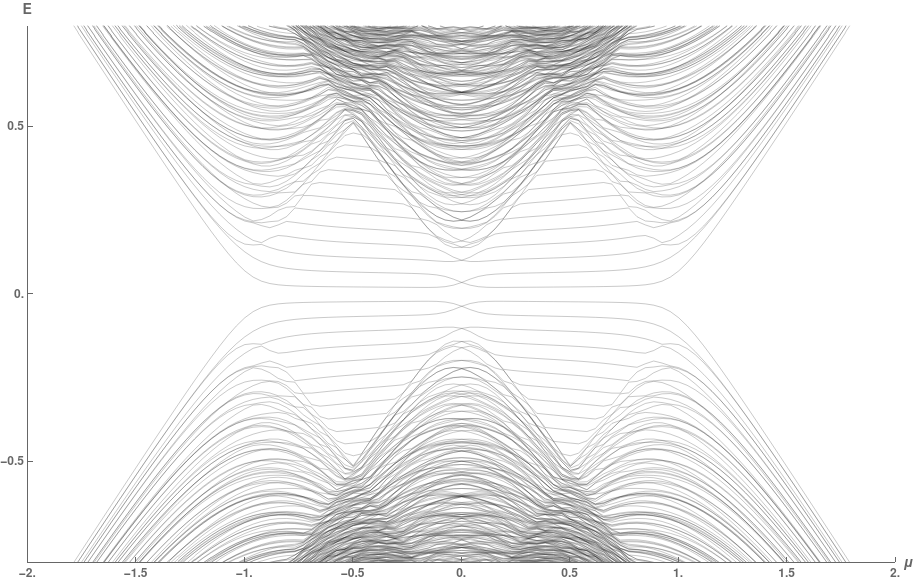
\includegraphics[width=\linewidth]{imgs/Spectrum_nP_nPeriodic.png}
    \caption{Spectrum for periodic boundary conditions and $t=\frac{1}{4}, \Delta = 1$. the axes where shifted to the edge to improve visibility of roots.}
    \label{fig:Spectrum_nP_nPeriodic}
\end{figure}
\pagebreak
\subsection{Vortices}
As \secref{sec:VBS} predicts zero-energy bound states in vortices, we begin to introduce pots in the chemical potential and Phase winding of the order parameter around them and analyse the spectrum for the expected roots. 
\begin{figure} [H]
\centering
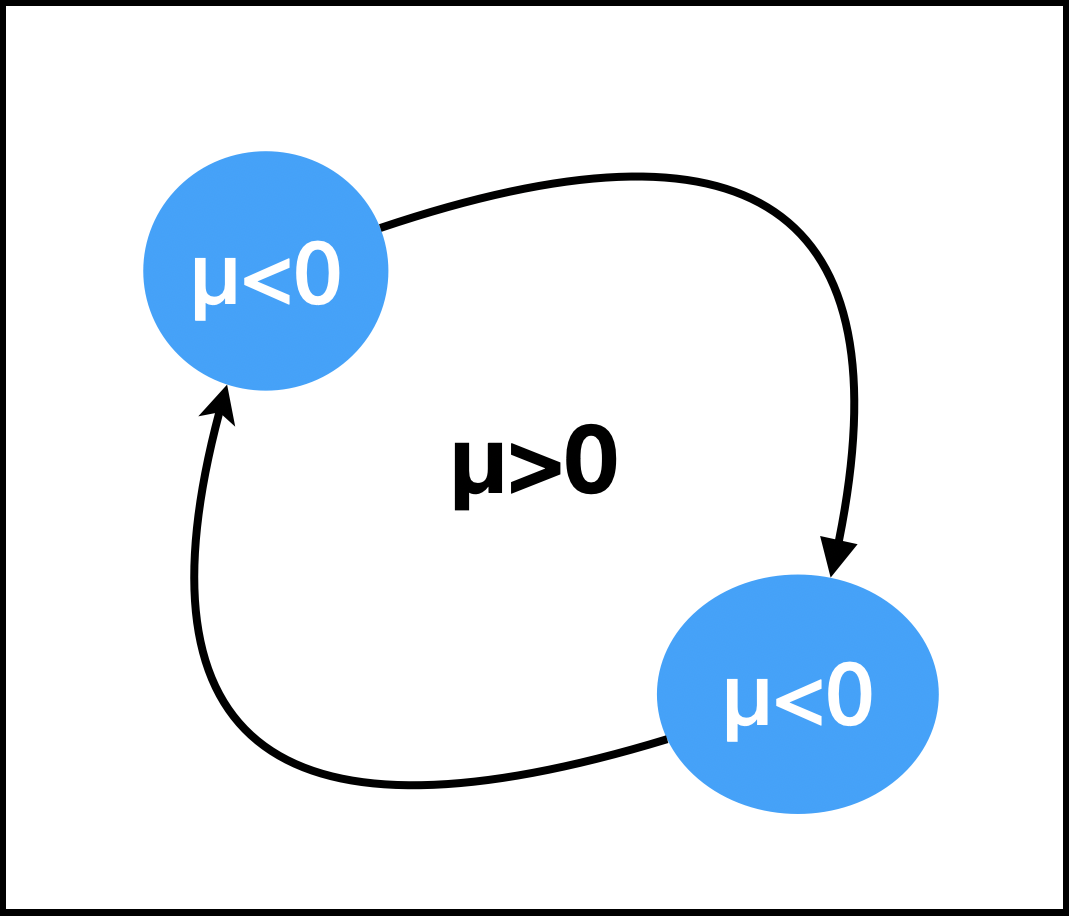
\includegraphics[width=0.2\linewidth]{imgs/Chem_Theory.png}
  \caption{Plot of discrete pots in the chemical potential and a circular exchange path}
  \label{fig:VortMuRot}
\end{figure}
\subsubsection{Chemical Potential}
In general, the chemical potential depends on time and space. From the theory, we know that, for zero-energy modes to form, the outside and inside of the pots needs to be in topologically different regimes, so the chemical potential is chosen accordingly. The theory further suggests the choice of the topologically trivial regime inside the pot and either the chiral+ or chiral- regime outside see \figref{fig:Phase_Diagramm}. However, we explore all cases. In practice, the chemical potential is below zero inside and above zero outside, or the other way round, and the chemical potential is then shifted globally by $\mu \rightarrow \pm 4t $ to realise a specific regime, as can be seen in \figref{fig:Phase_Diagramm+-4t}. We use pots with the radius $R$ of the $\mu = 0 $ transition and vortices the points $(V_x^i,V_y^i)$. The chemical potential can be changed continuously or discretely. So we use both discrete pots, where the chemical potential is locally constant and only changes signs at the edge and pots where the chemical potential follows a Gaussian function.
In the Discrete case, the chemical potential follows 
$$
\mu_{x,y} = 
\begin{cases}
-\mu_0 \pm 4t  & \min_i((x-V_x^i)^2+(y-V_y^i)^2) < R^2 \\
\mu_0 \pm 4t &  \min_i((x-V_x^i)^2+(y-V_y^i)^2) > R^2 
\end{cases}\text{.}
$$
Whereas the chemical potential for Gaussian pots is of the from
$$
\mu_{x,y} = \mu_0 - 2 \mu_0 \sum_i \exp \left( \frac{\ln(0.5) }{ R^2 }((x  - V_x^i)^2 +(y - V_y^i)^2 ) \right) \pm 4t \text{.}
$$
\begin{figure}[H]
\centering
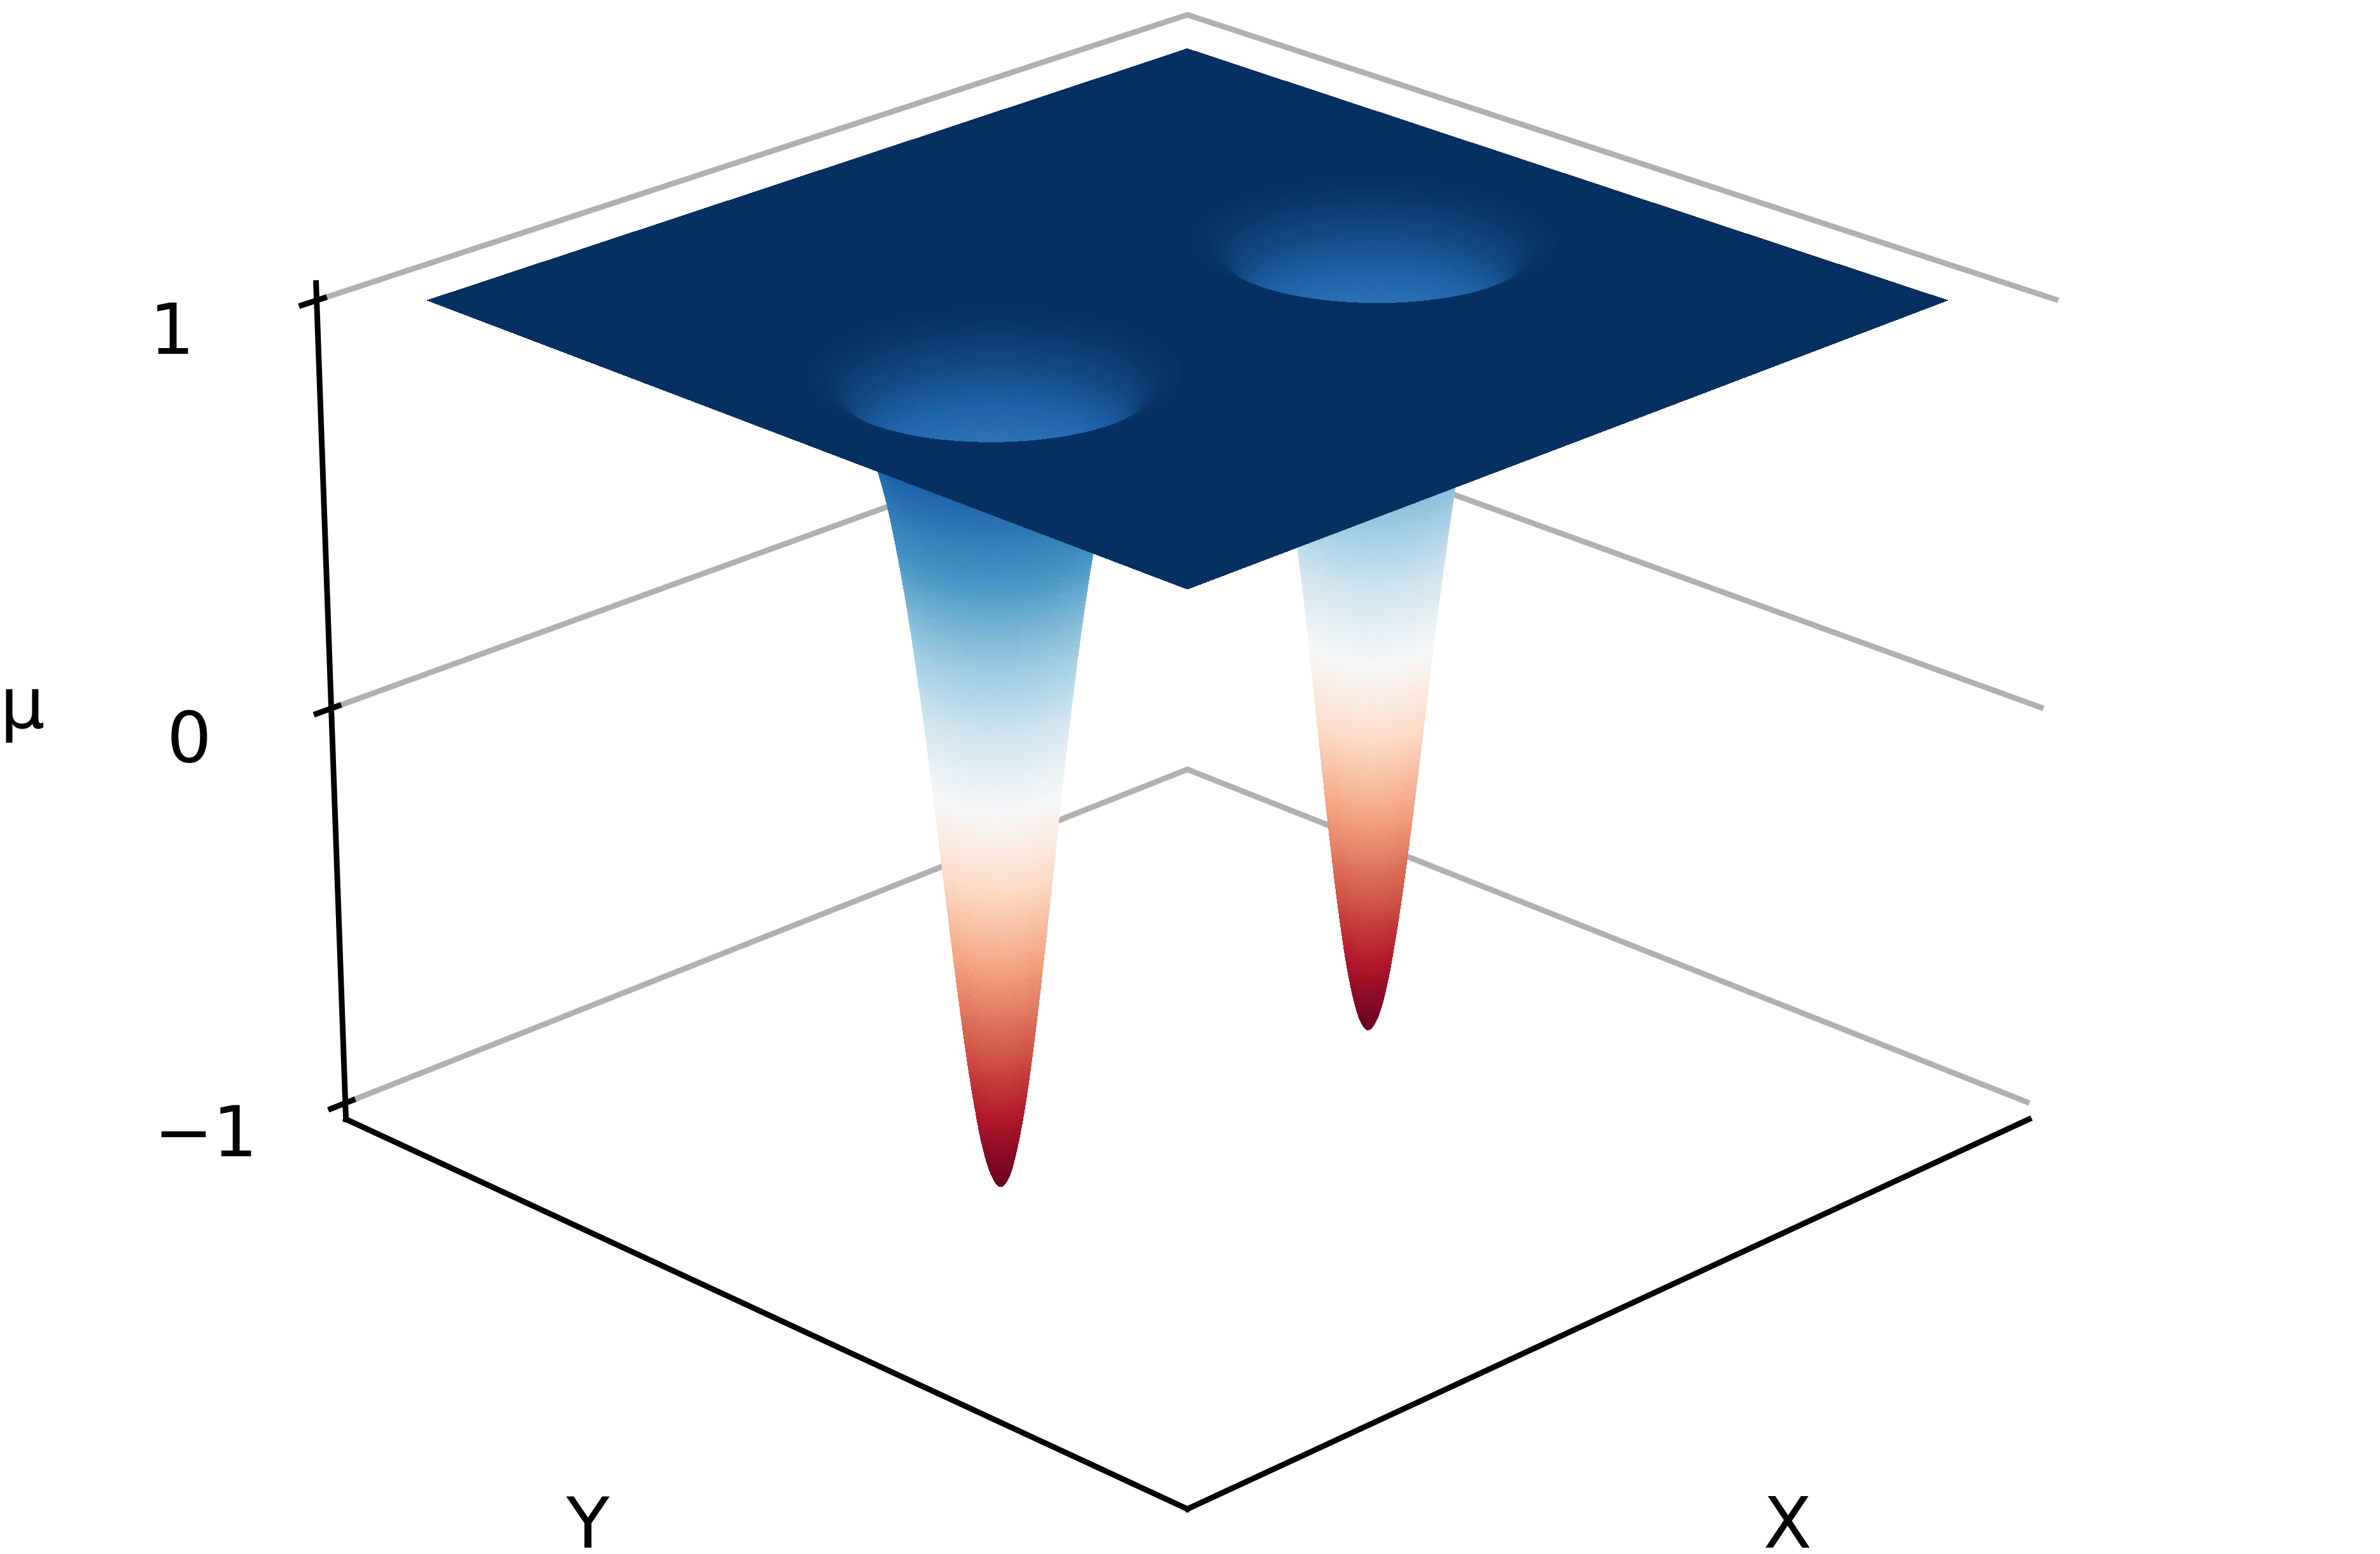
\includegraphics[width=0.5\linewidth]{imgs/Mu_Plot.png}
  \caption{Plot of the chemical potential of a Gaussian vortex pair in real space, with pots along the x axis at $V_x^1=G/4,V_x^2=-G/4, V_y^{1/2} = 0$ and a radius $R = G/8$}
  \label{fig:MuVorts}
\end{figure}
\pagebreak
We plot the eigenvalues for fixed $t=14,\Delta = 1$ along the $\mu$ axis and observe the spectrum of this system without periodic boundary conditions, for discrete pots see \figref{fig:Spectrum_nP_nPeriodic_Vorts} and for contineous pots see \figref{fig:Spectrum_nP_nPeriodic_gaussVorts}
\begin{figure}[H]
\centering
\begin{minipage}[c]{\textwidth}
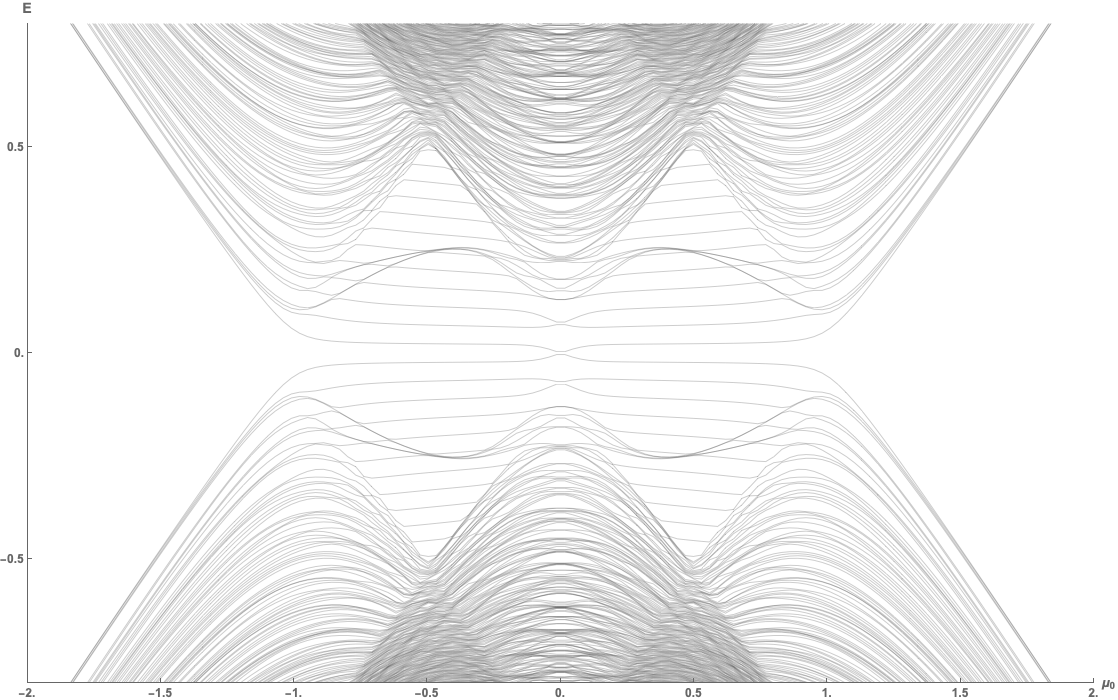
\includegraphics[width = \linewidth]{imgs/Spectrum_nP_nPeriodic_Vorts.png}
\caption{For discrete vortices the spectrum is similar as without vortices. $t=\frac{1}{4}, \Delta = 1, \mu_0 = -2, R = grid/8$}
\label{fig:Spectrum_nP_nPeriodic_Vorts}
\end{minipage}\\
\begin{minipage}[c]{\textwidth}
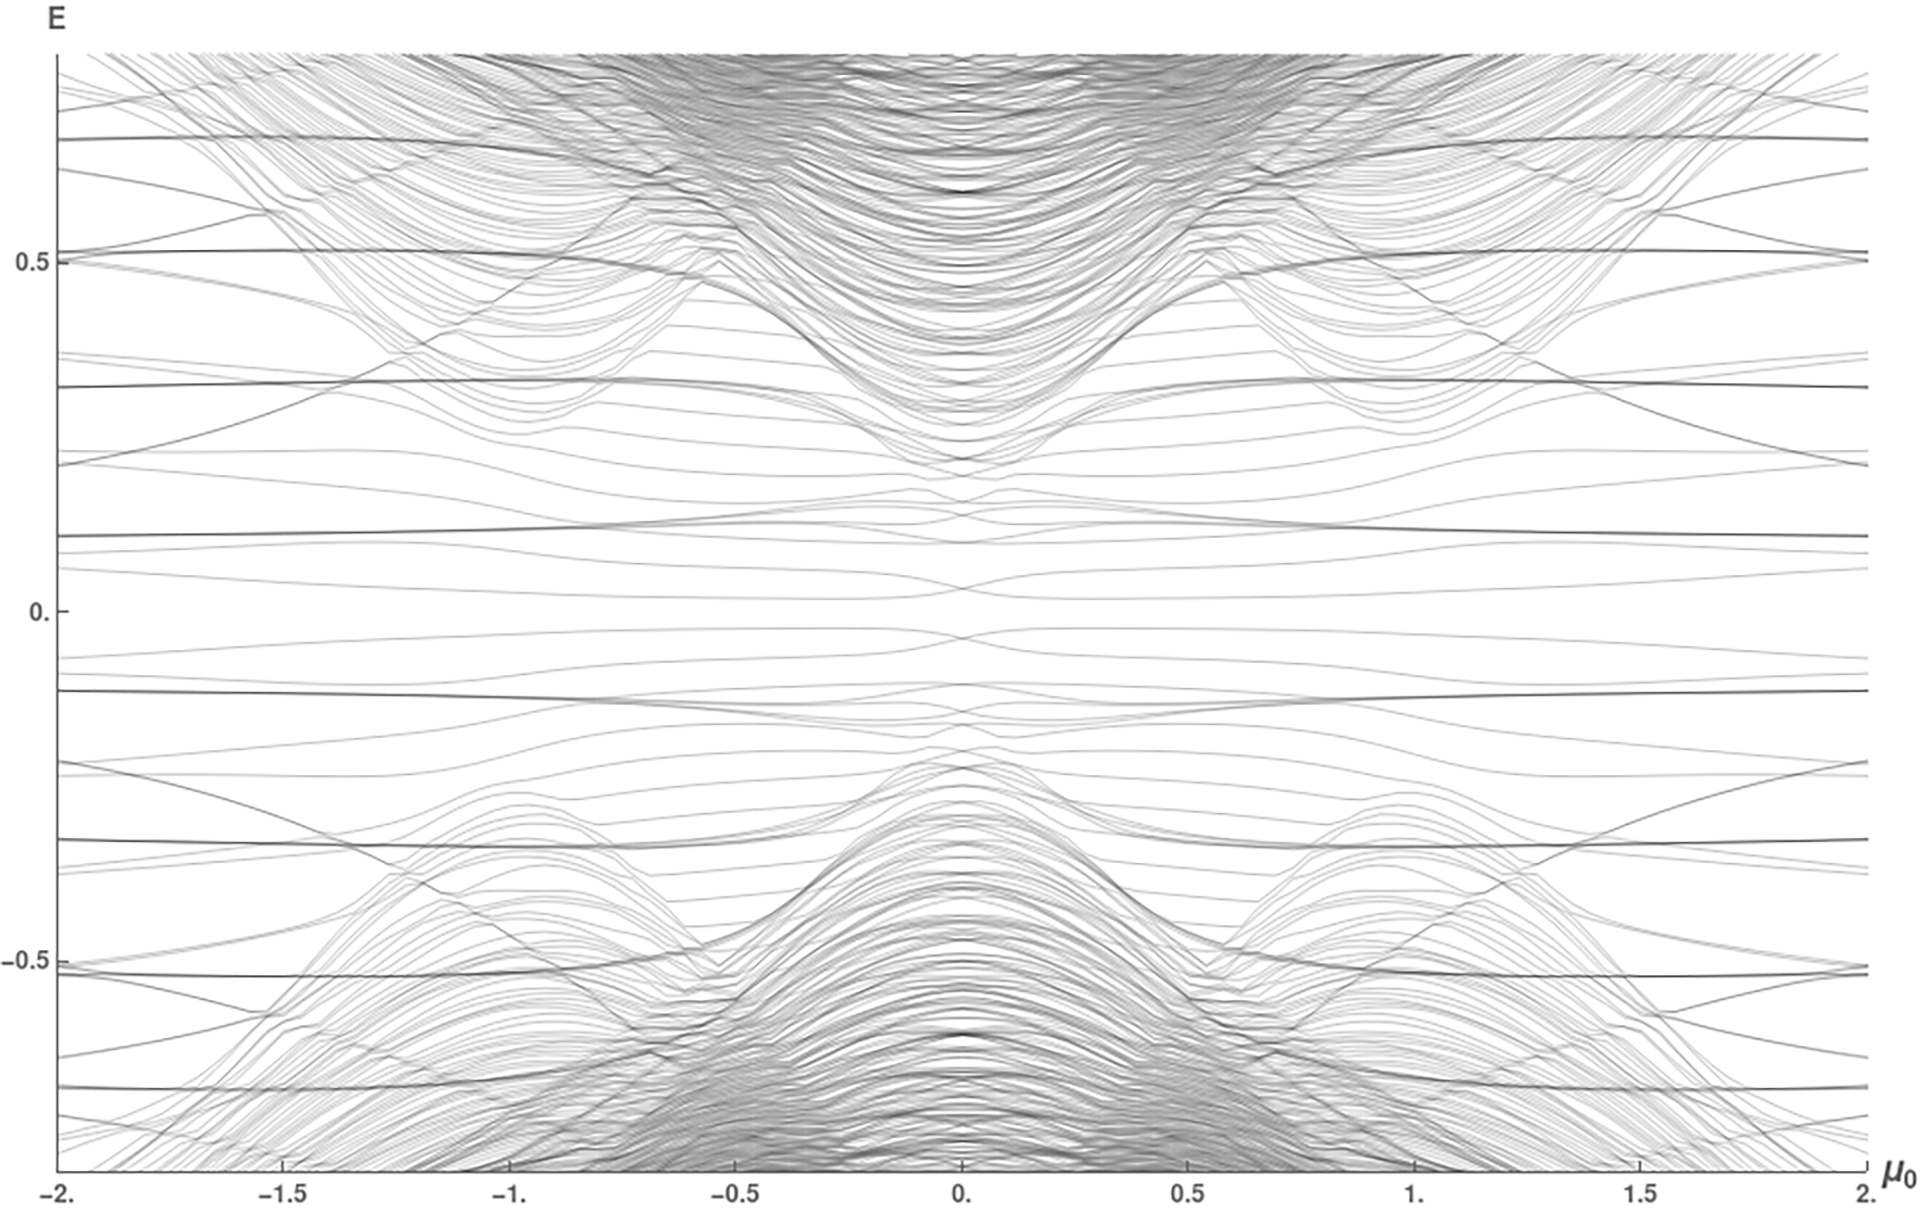
\includegraphics[width = \linewidth]{imgs/Spectrum_nP_nPeriodic_gaussVorts.png}
\caption{For Gaussian vortices the spectrum shows new low energy states as the chemical energy vanishes close to the boundary $t=\frac{1}{4}, \Delta = 1, \mu_0 = -2, R = grid/8$}
\label{fig:Spectrum_nP_nPeriodic_gaussVorts}
\end{minipage}
\end{figure}
\pagebreak
\subsubsection{Phase Winding}
When only the Chemical Potential is present and the Order Parameter is kept fixed in space, the spectrum inside the gap is symmetric and gaped around zero.
However, this spectrum has no zero energy modes.
To get our desired non-abelian zero-energy Majorana modes we have to introduce a phase winding around the pots hence make them vortices. In practice this is done by multiplying a phase factor $\Delta^i_{m.n}$ for each vortex $i$ at a pair of neighbouring sites $m$ and $n$:
$$
\Delta^i_{m.n} = \frac{1}{2} \left((m_x+n_x - 2 V^i_x) + i (m_y+n_y - 2 V^i_y))\right)
$$
$$ \Delta_{m,n} = \Delta_0 \prod_i 
\begin{cases}
0 & \Delta^i_{m,n}= 0\\
\frac{\Delta^i_{m,n}}{|\Delta^i_{m,n}|} & \Delta^i \neq 0
\end{cases}
$$
 \begin{figure}[H]
\centering
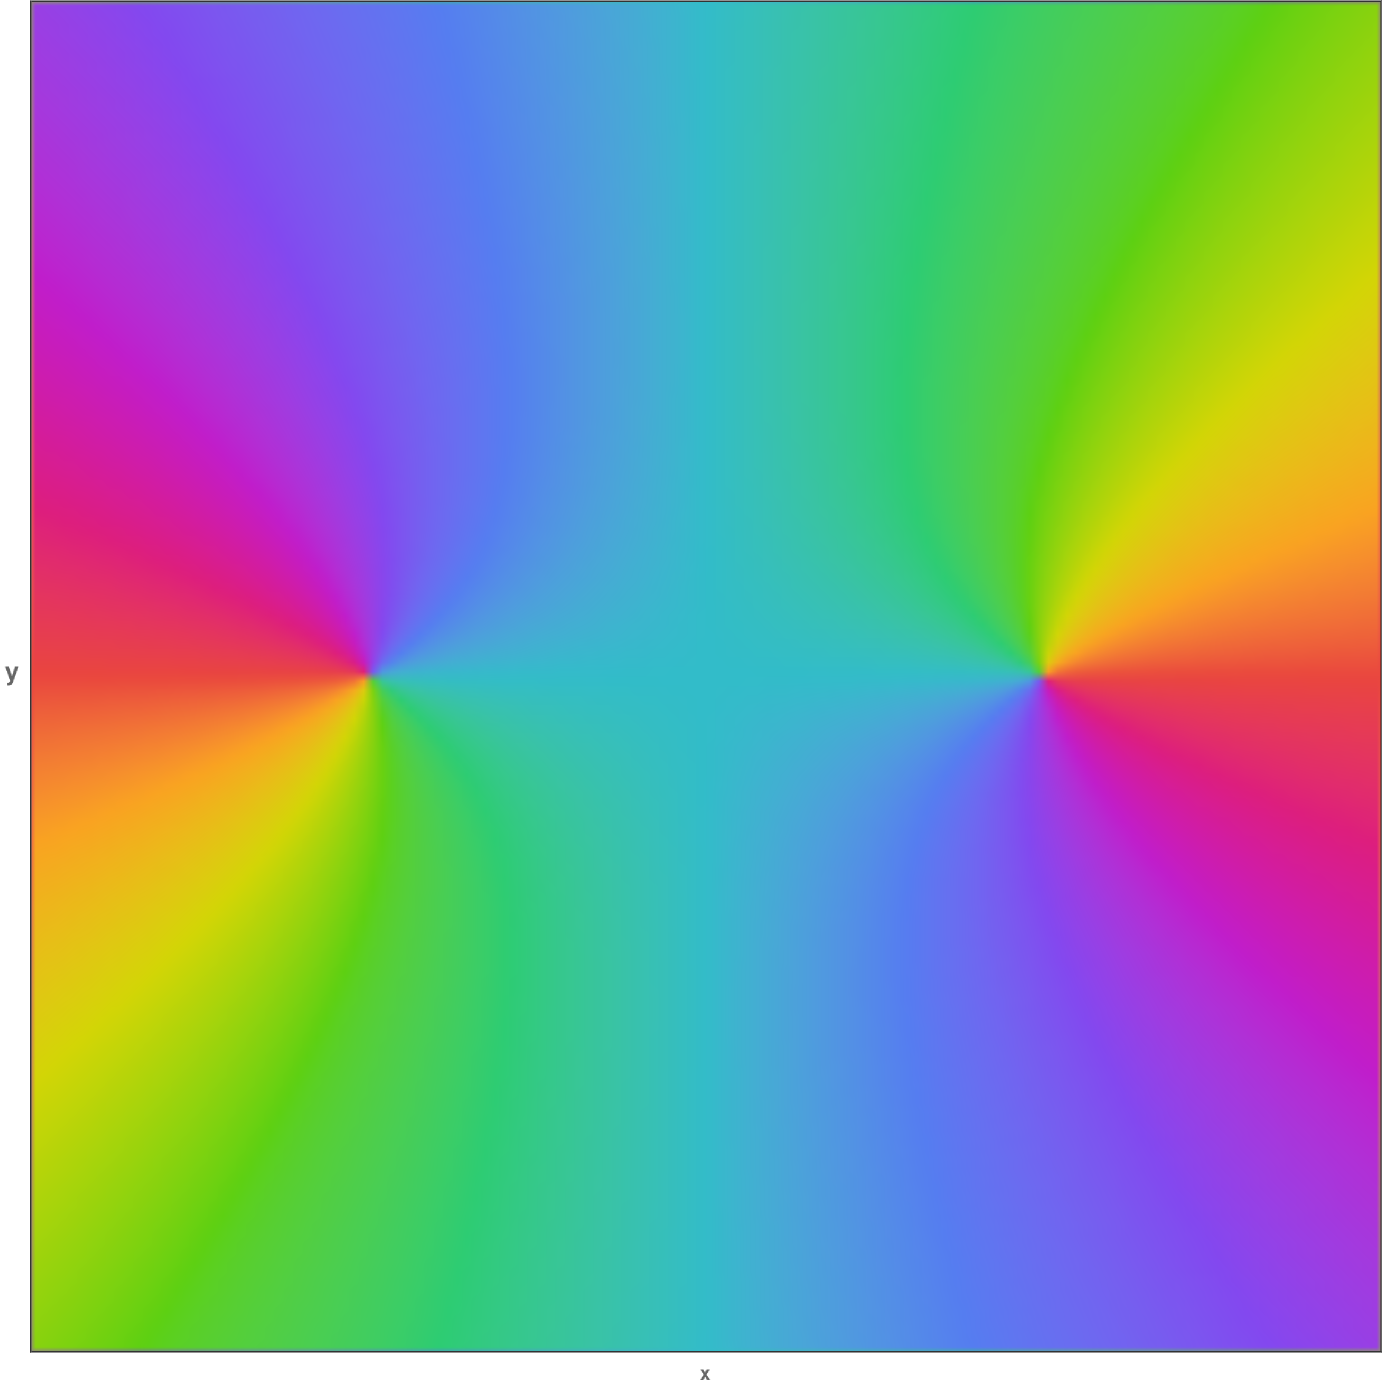
\includegraphics[width=0.3\linewidth]{imgs/Phase_Winding.png}
  \caption{Complex plot of phase winding around vortices}
  \label{fig:Phase_Winding}
\end{figure}
\begin{figure}[H]
    \centering
    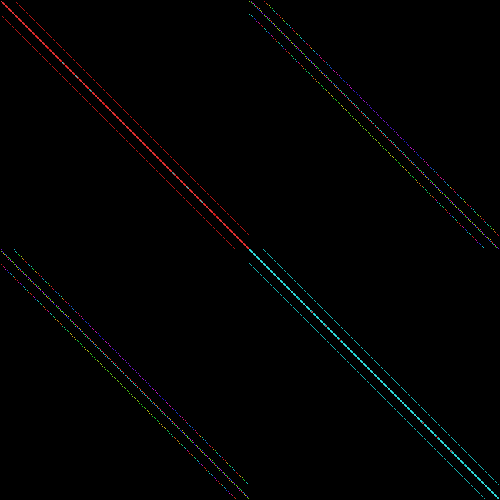
\includegraphics[width=0.3\linewidth]{imgs/Matrix_nP_Phase_Gauss.png}
    \caption{Matrix with phase winding and gaussian vorices. $t=\frac{1}{4}, \Delta = 1, \mu = -2$}
    \label{fig:MatrixnPPhGauss}
\end{figure}
In \figref{fig:MatrixnPPhGauss} the phase-winding of the $M$ matrix can be seen as a rainbow pattern along the $B$ matrix block diagonals. The Gaussian pots appear as small dots on the diagonal with opposite sign (red/cyan) as the sign of the chemical potential changes. We show the emerging spectrum for discrete vortices in \figref{fig:Spectrum_P_nPeriodic_Vorts} and for Gaussian vortices in \figref{fig:Spectrum_P_nPeriodic_gaussVorts}
\begin{figure}[H]
\begin{minipage}[c]{\textwidth}
\centering
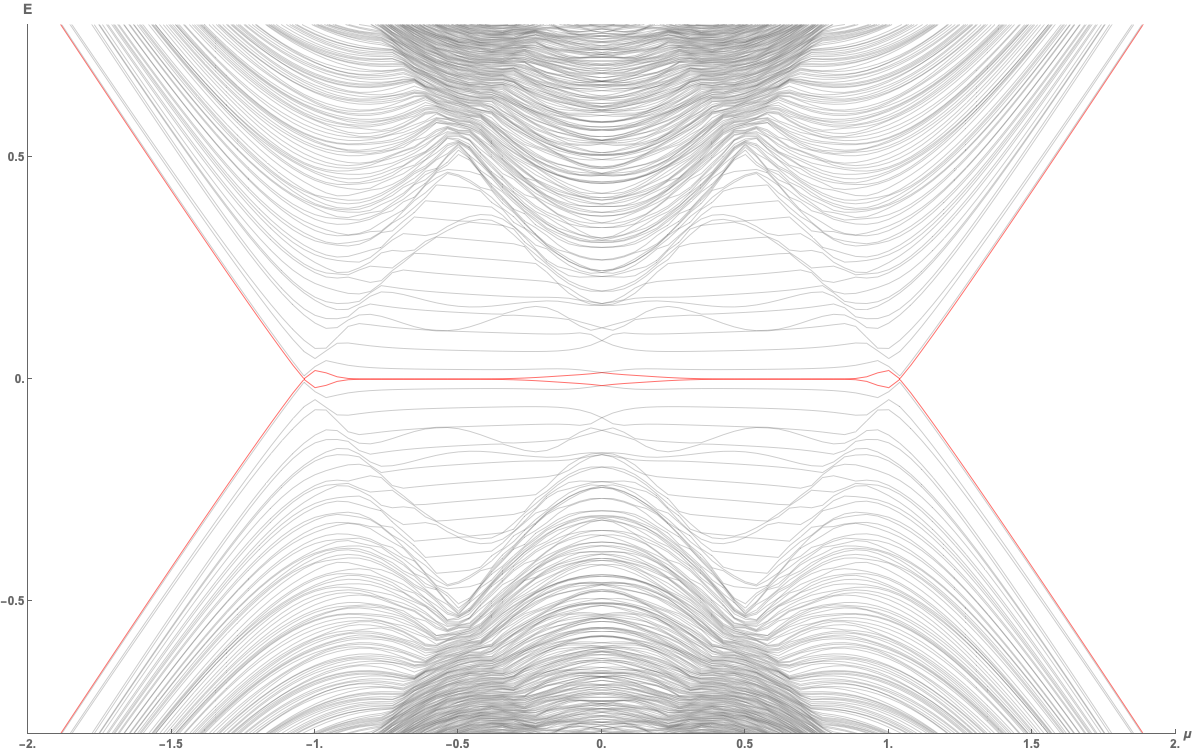
\includegraphics[width = \linewidth]{imgs/Spectrum_P_nPeriodic_Vorts.png}
\caption{Spectrum for discrete vortices, zero energy mode coloured in red . $t=\frac{1}{4}, \Delta = 1, \mu_0 = -2, R = Grid/8$ witout a $\pm 4t$ shift}
\label{fig:Spectrum_P_nPeriodic_Vorts}
\end{minipage}\\
\begin{minipage}[c]{\textwidth}
\centering
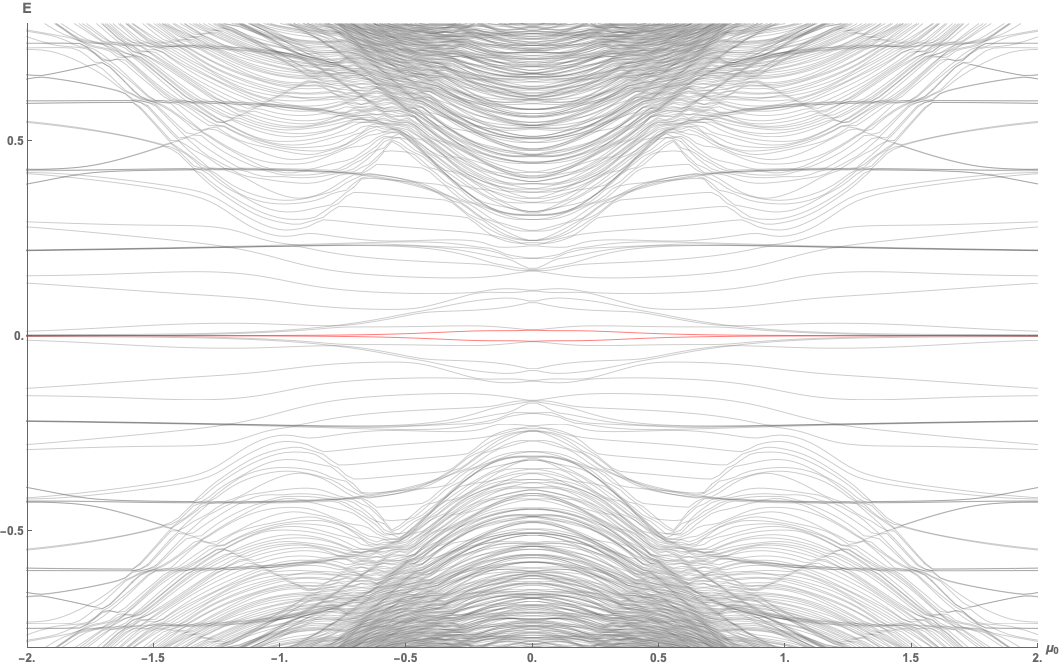
\includegraphics[width = \linewidth]{imgs/Spectrum_P_nPeriodic_gaussVorts.png}
\caption{Spectrum for Gaussian vortices, zero energy mode coloured in red  $t=\frac{1}{4}, \Delta = 1, R = Grid/8$ depending on $\mu_0$ witout a $\pm 4t$ shift}
\label{fig:Spectrum_P_nPeriodic_gaussVorts}
\end{minipage}
\end{figure}
As in this case no $\pm 4t$ shift is present, for $|\mu_0|<1 = 4<t|$ both the inside and the outside of the vortex are in different but topologically nontrivial regimes. We observe zero energy modes, in both cases and a mirror symmetrical spectrum along $\mu=0$.
For $|\mu_0|>1 = 4|t|$ the vortex has two phase transitions. In the case witout a $\pm 4t$ shift the chemical potential passes from the chiral+ to the chiral- regime at $\mu=0$, and at $\mu = \pm 4t$ the transition to the topologically trivial gregime. Thus enters a further critical region see \figref{fig:ChemMulti}.
\begin{figure}[H]
\begin{minipage}[c]{\textwidth}
\centering
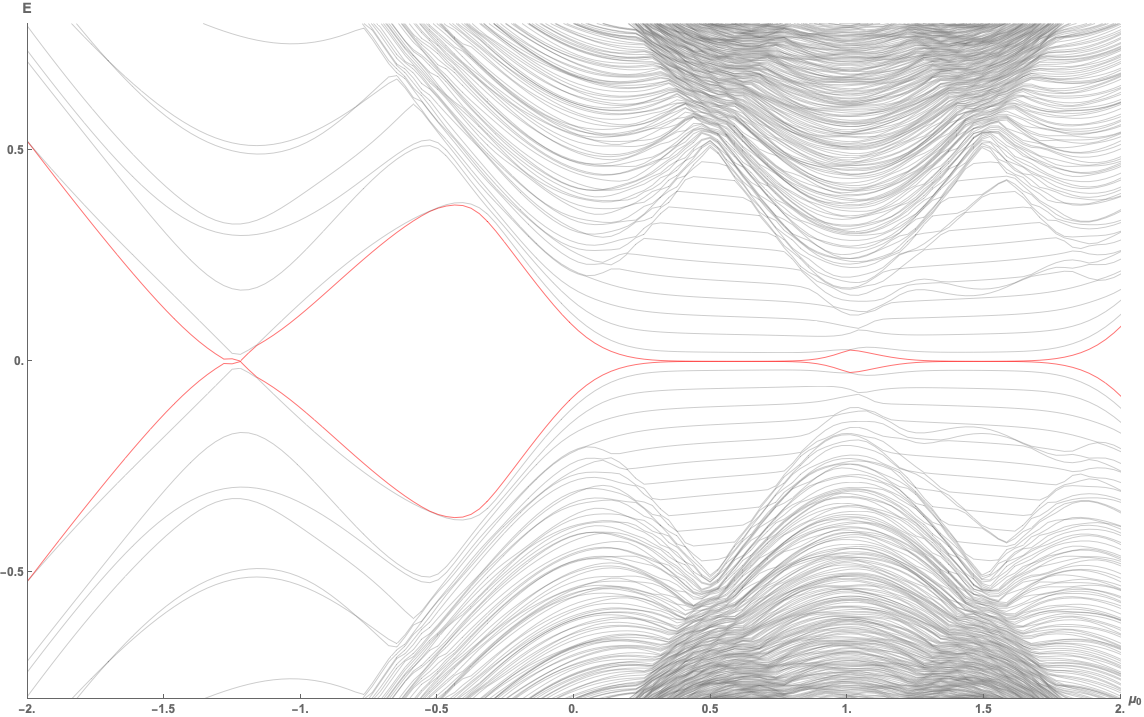
\includegraphics[width = \linewidth]{imgs/Spectrum_P_nPeriodic_Vorts-4t.png}
\caption{Spectrum for discrete vortices, zero energy mode coloured in red  $t=\frac{1}{4}, \Delta = 1, R = Grid/8$ depending on $\mu_0$ with a $-4t$ shift}
\end{minipage}\\
\begin{minipage}[c]{\textwidth}
\centering
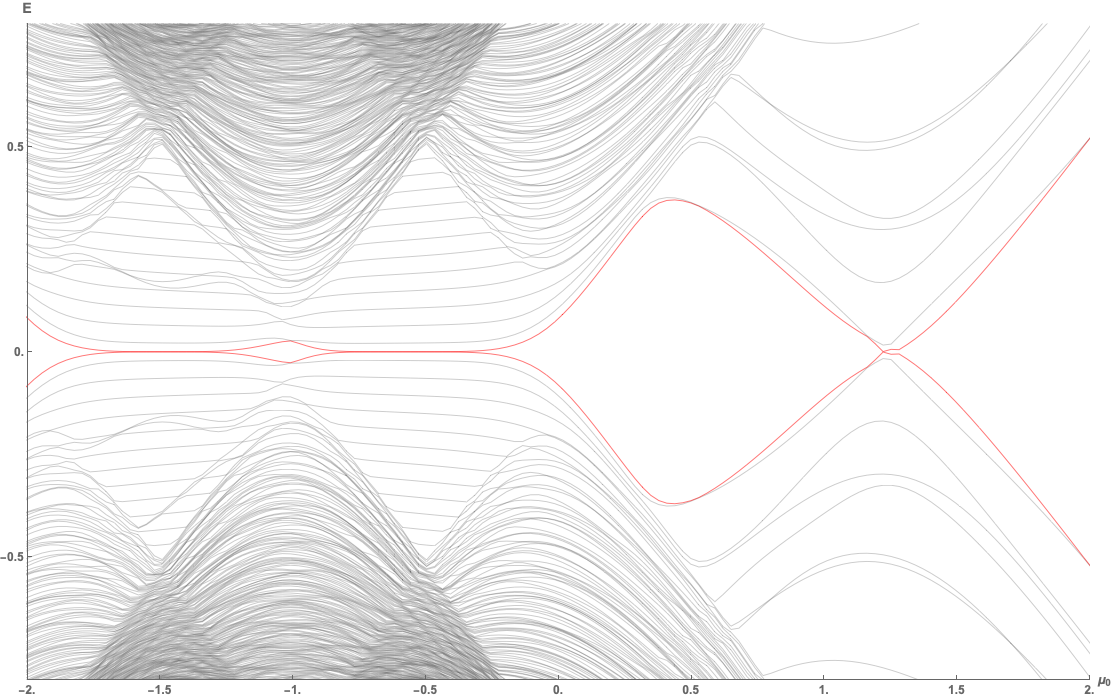
\includegraphics[width = \linewidth]{imgs/Spectrum_P_nPeriodic_Vorts+4t.png}
\caption{Spectrum for discrete vortices, zero energy mode coloured in red  $t=\frac{1}{4}, \Delta = 1, R = Grid/8$ depending on $\mu_0$ with a $+4t$ shift}
\end{minipage}
\end{figure}
\begin{figure}[H]
\begin{minipage}[c]{\textwidth}
\centering
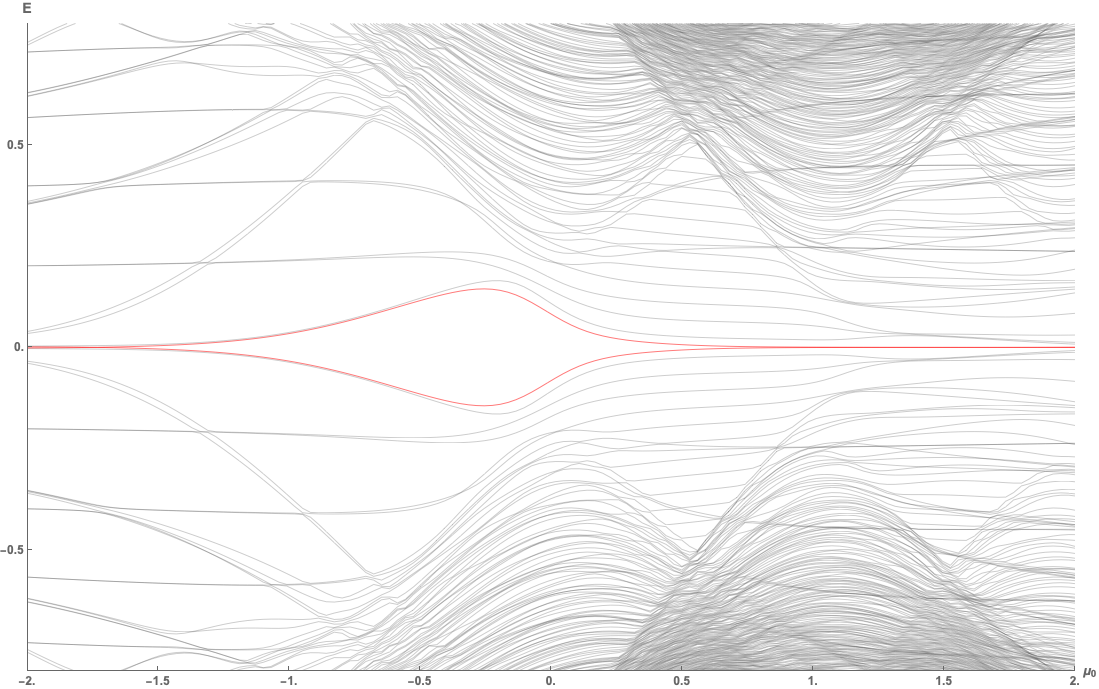
\includegraphics[width = \linewidth]{imgs/Spectrum_P_nPeriodic_gaussVorts-4t.png}
\caption{Spectrum for Gaussian vortices, zero energy mode coloured in red  $t=\frac{1}{4}, \Delta = 1, R = Grid/8$ depending on $\mu_0$ with a $-4t$ shift}
\end{minipage}\\
\begin{minipage}[c]{\textwidth}
\centering
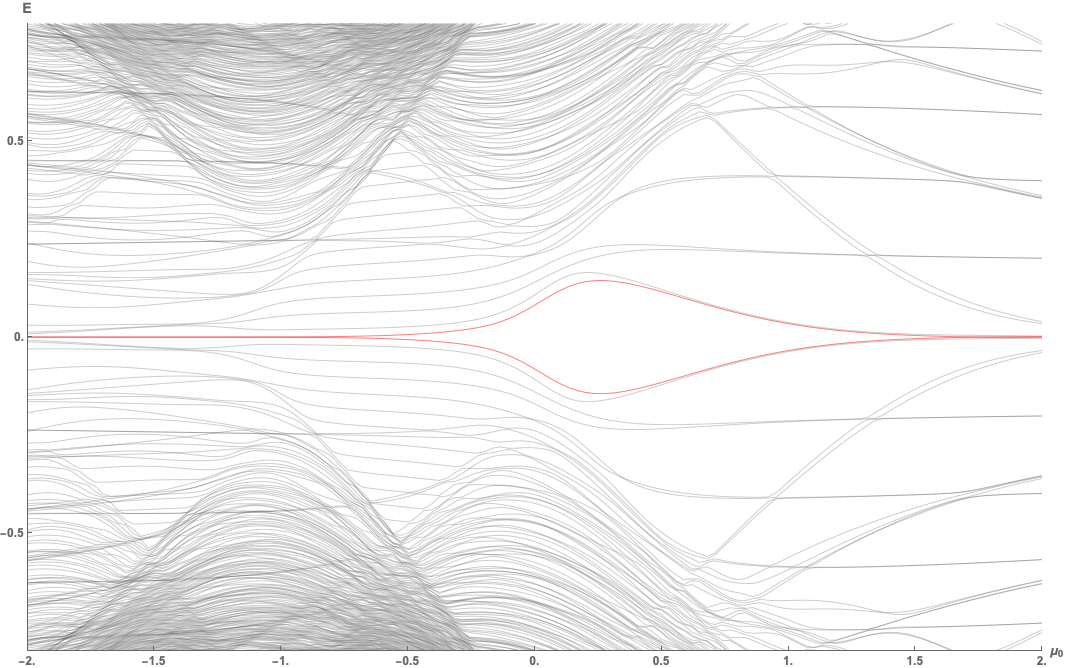
\includegraphics[width = \linewidth]{imgs/Spectrum_P_nPeriodic_gaussVorts+4t.png}
\caption{Spectrum for Gaussian vortices, zero energy mode coloured in red  $t=\frac{1}{4}, \Delta = 1, R = Grid/8$ depending on $\mu_0$ with a $+4t$ shift}
\end{minipage}
\end{figure}
In the case of a chemical potential that is shifted by $\pm 4t$, only one side is in the topological regime, We observe that the topological phase has to be on the outside of the vortex, for a zero energy mode to exist. We further observe multiple phase transitions again for $|\mu_0| > 4 |t|$ \figref{fig:ChemMulti}. The spectrum is flipped for the $+4t$ and $-4t$ shifted cases but the phase transition is different. 
Once the vortex passes from chiral+ to trivial and once from chiral- to trivial.
In all cases with Gaussian vortices, we observe that the energy-splitting vanishes much slower when entering the right regime configuration than for discrete vortices. Therefore, we will continue only with discrete vortices.
\begin{figure}
    \centering
    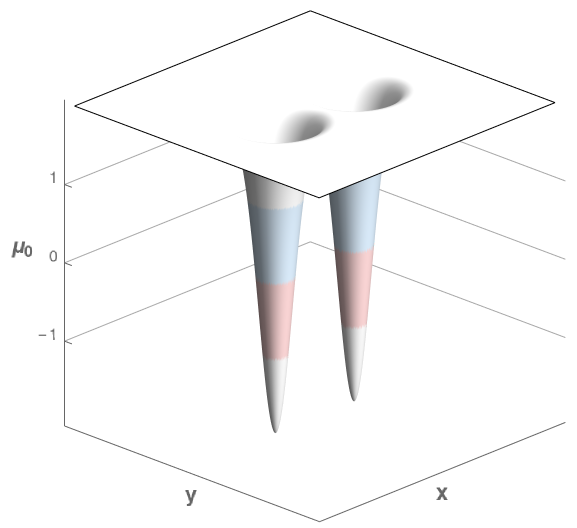
\includegraphics[width=0.4\linewidth]{imgs/ChemPotMultiphase.png}
    \caption{Gaussian chemical potential extending over all different topological regions.
    Coloured white trivial, chrial+ blue, chiral- red, for $t=-\frac{1}{2},\Delta=1$}
    \label{fig:ChemMulti}
\end{figure}
We further compare how the spectrum changes as a function of the vortex radius:
\begin{figure}[H]
 \centering
\begin{tabular}{cc}
    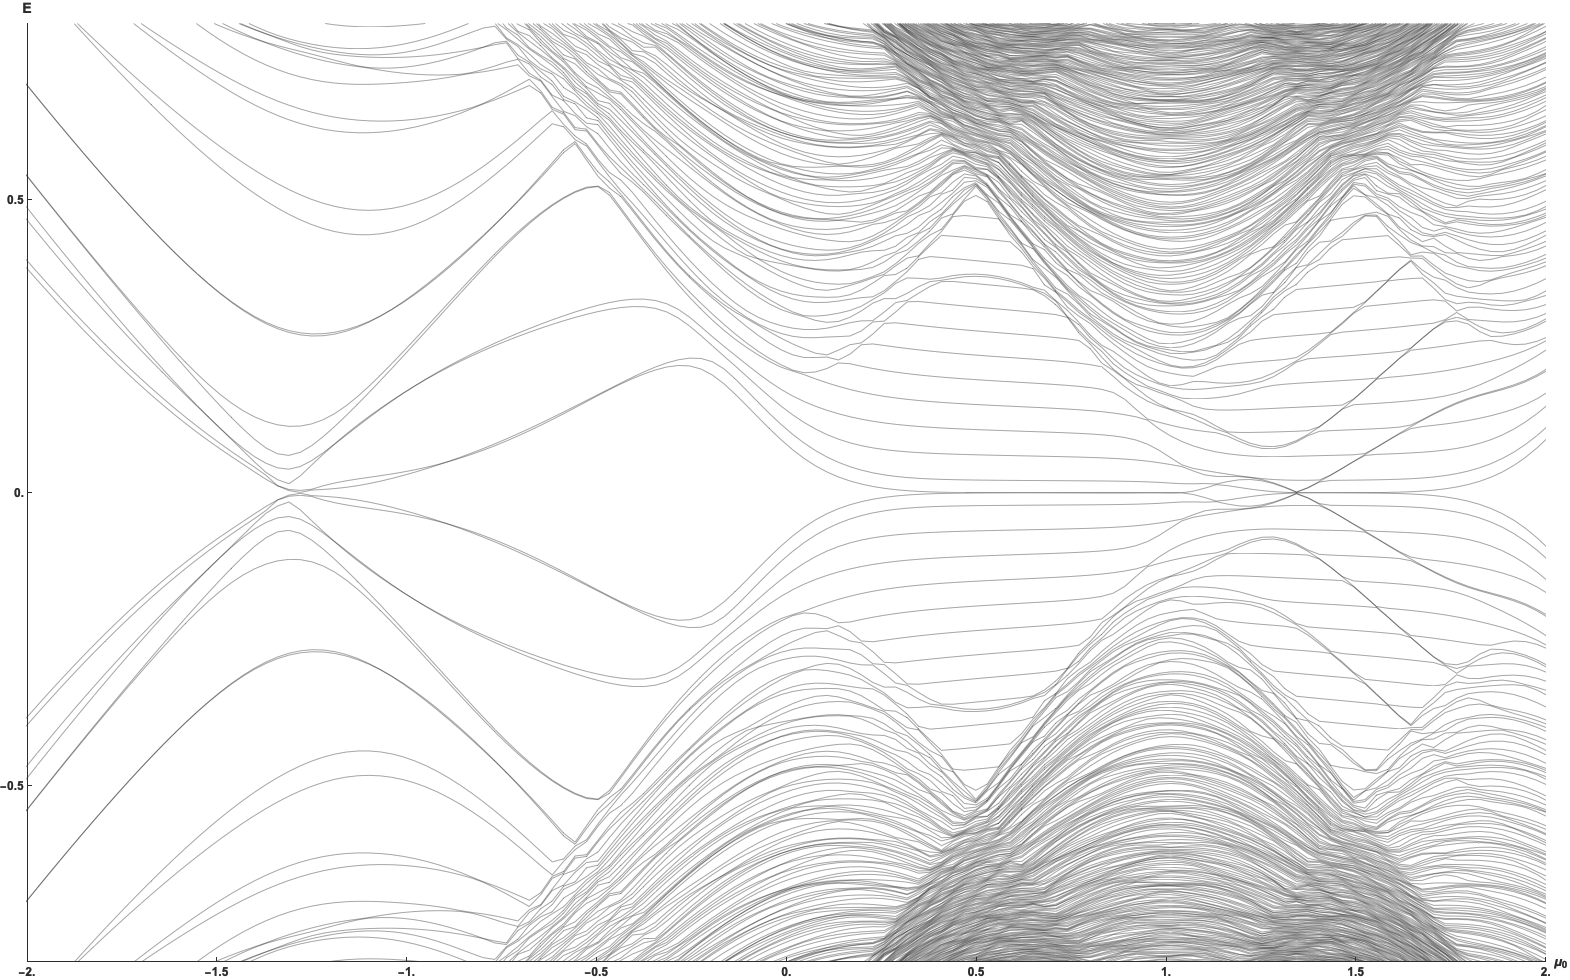
\includegraphics[width=0.5\textwidth]{imgs/Spectrum_G2 copy.png}
    & 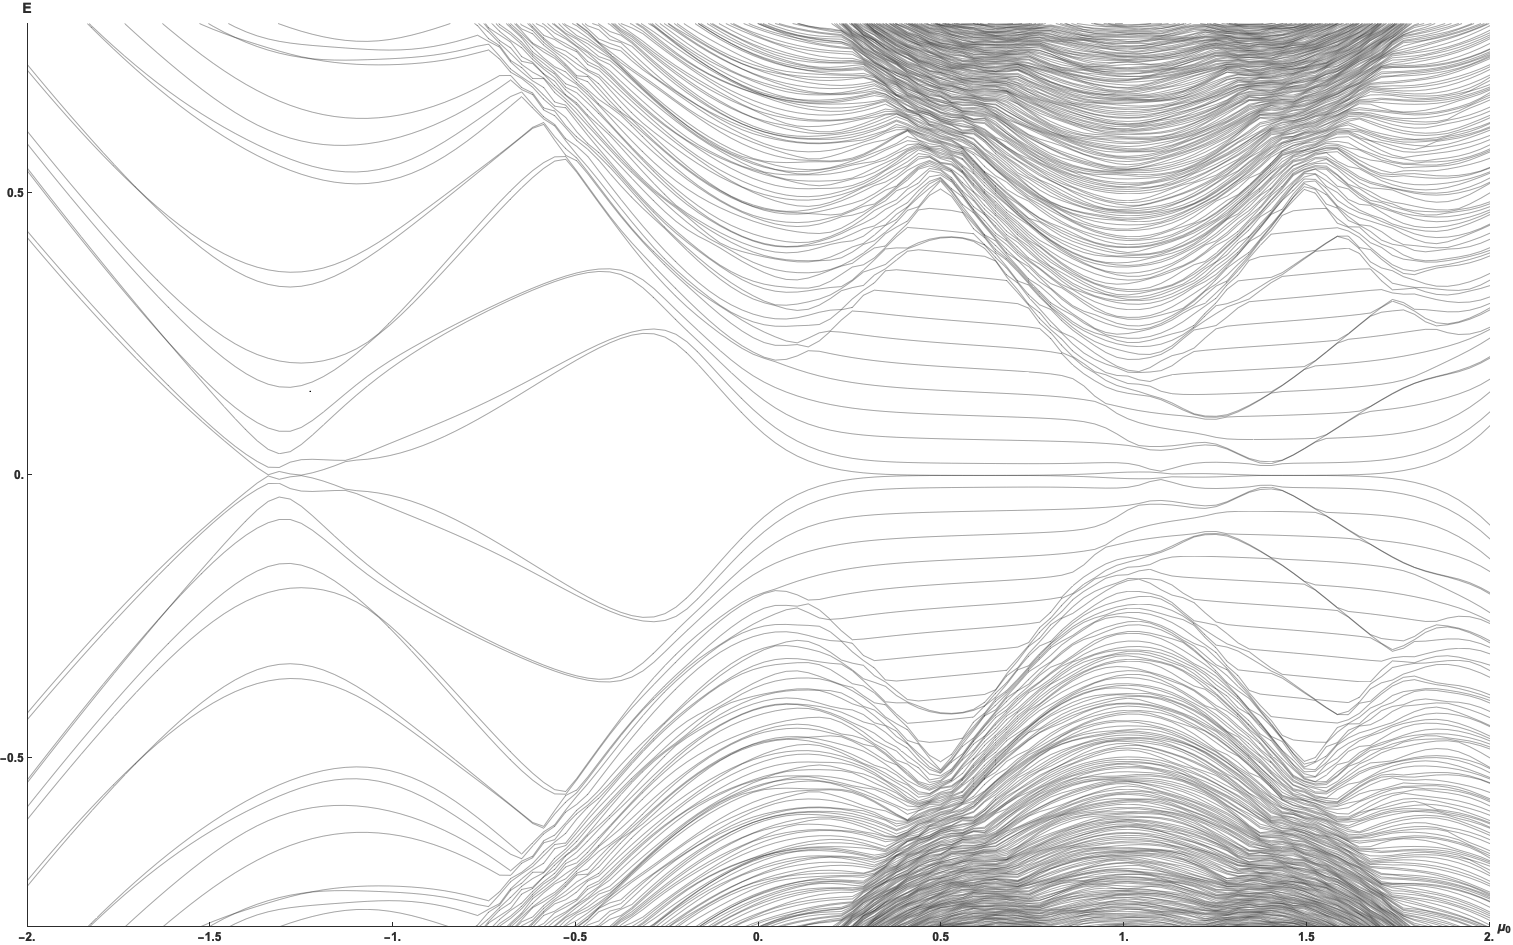
\includegraphics[width=0.5\textwidth]{imgs/Spectrum_G6 copy.png}\\
     $R = G/2$ &$R = G/6$\\
    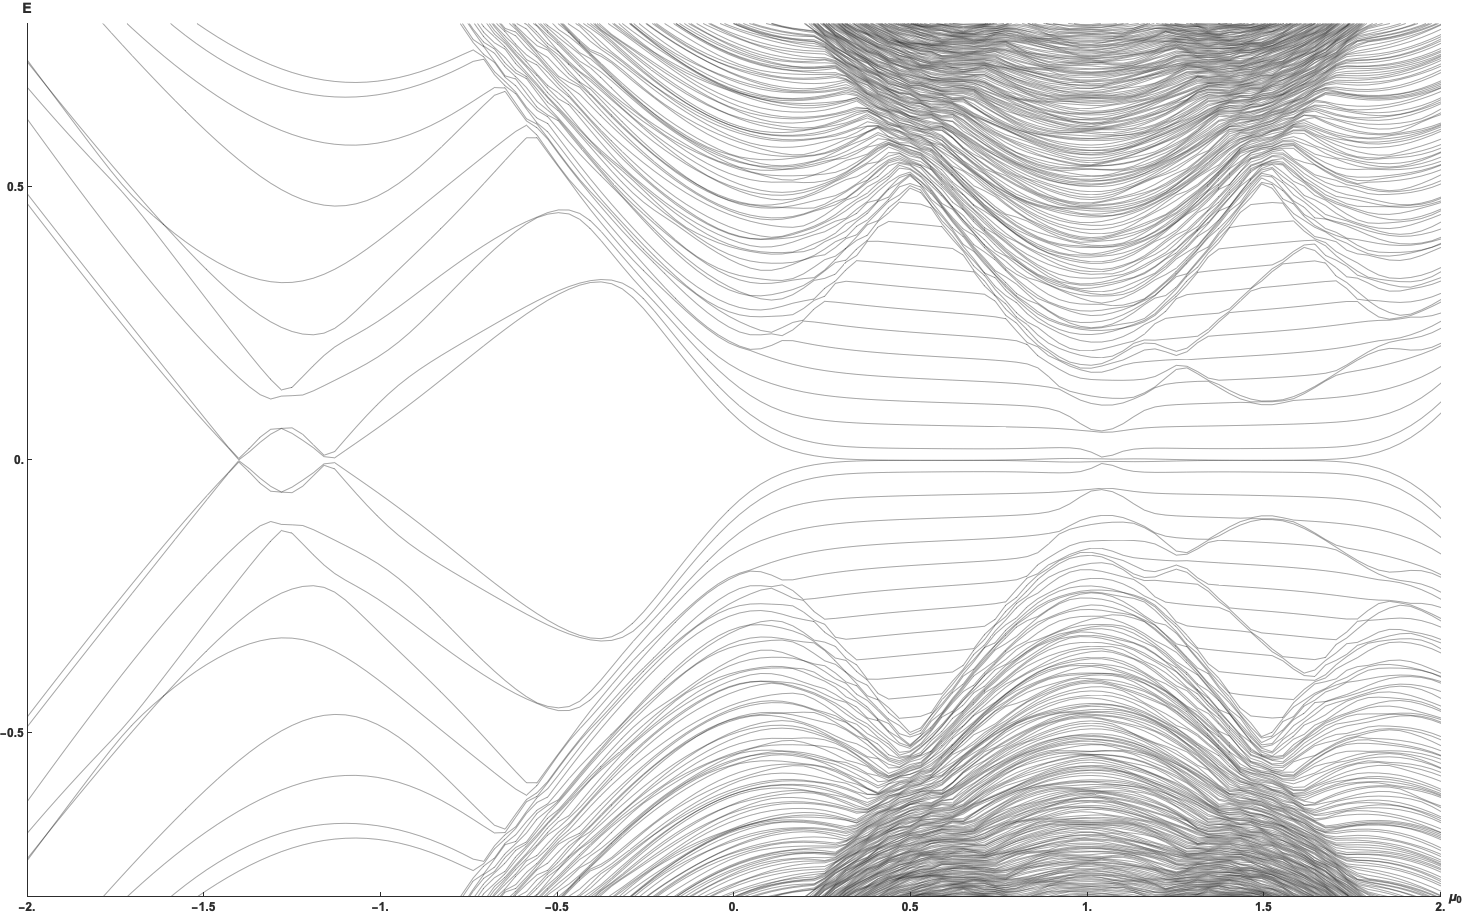
\includegraphics[width=0.5\textwidth]{imgs/Spectrum_G10 copy.png}&
    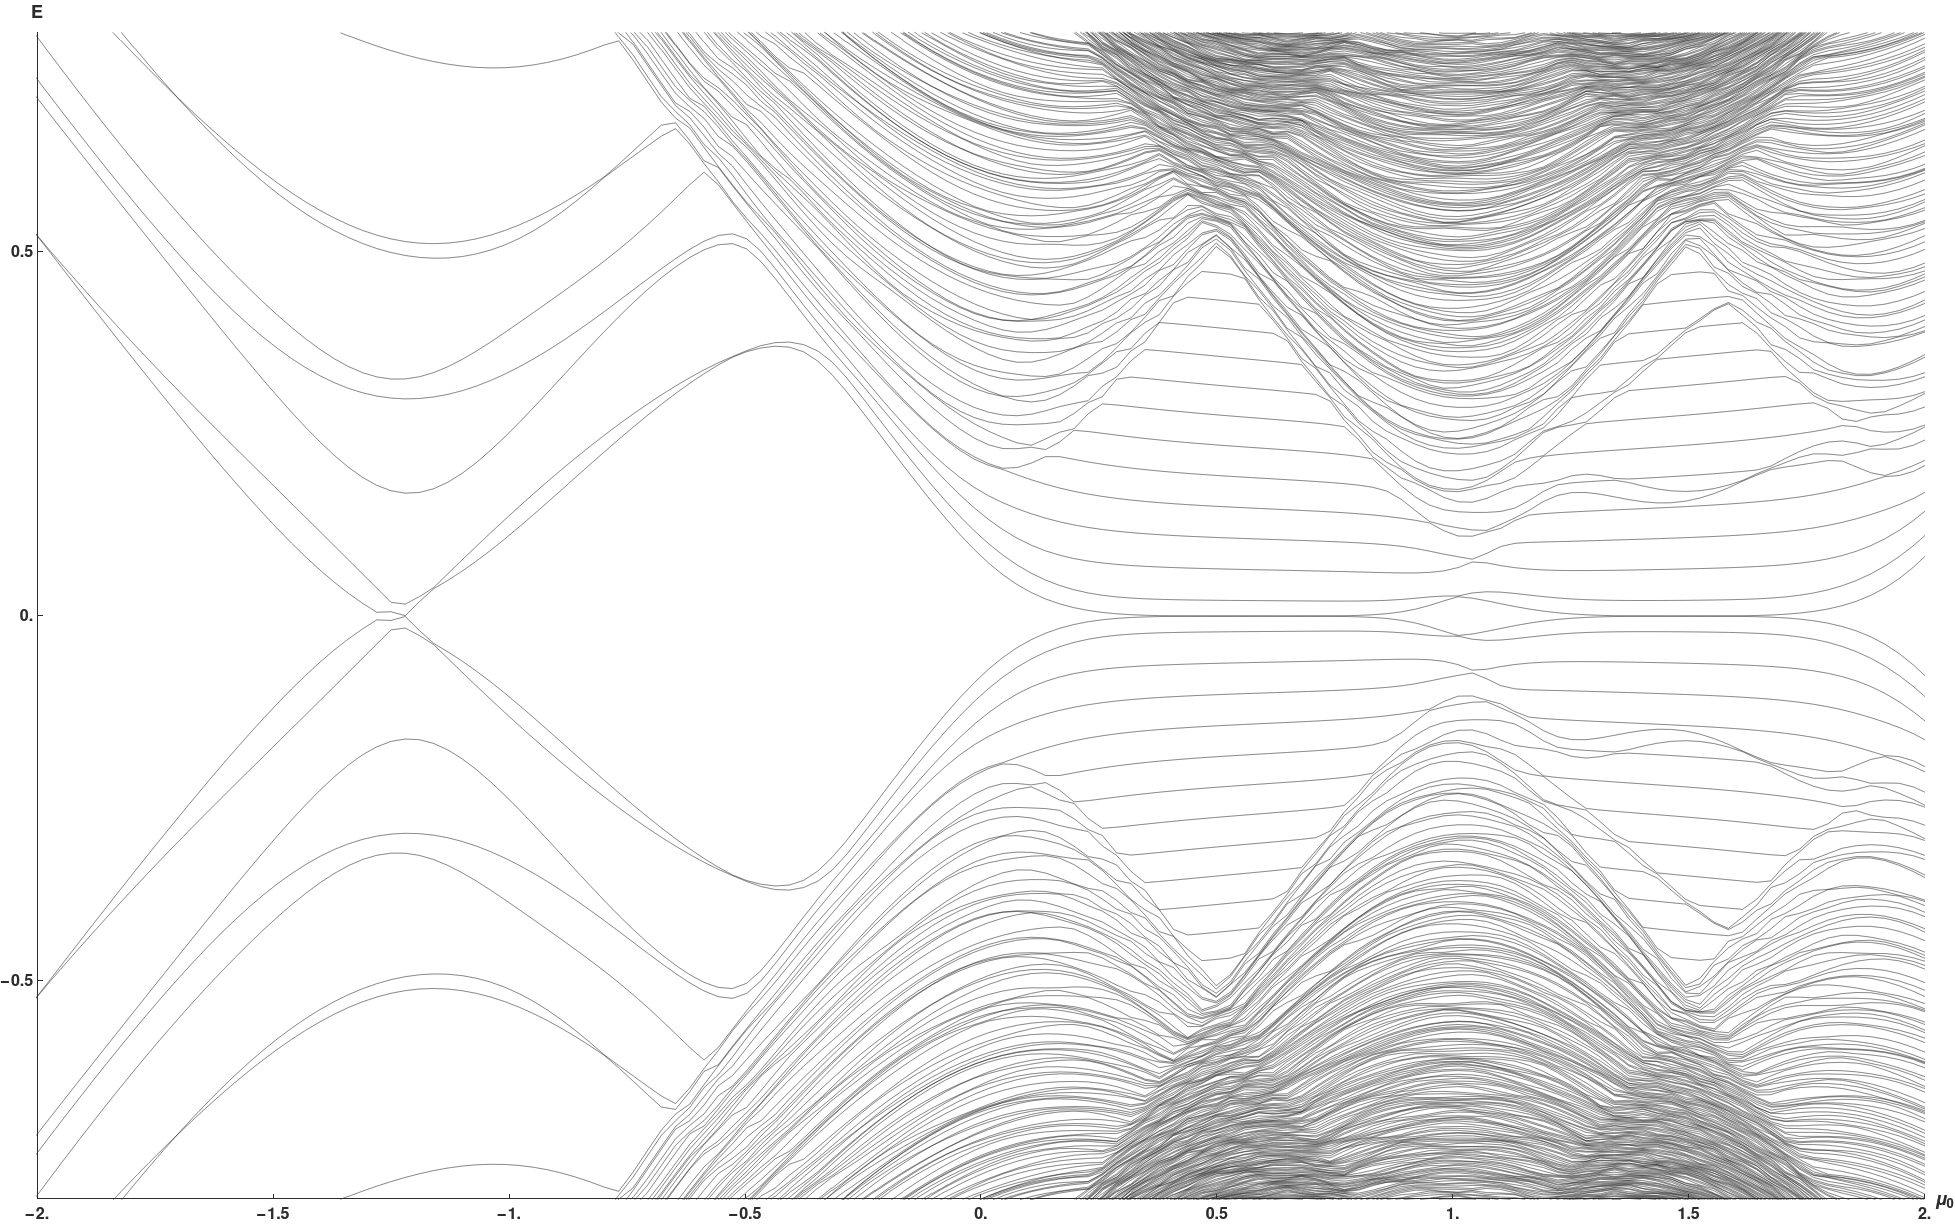
\includegraphics[width=0.5\textwidth]{imgs/Spectrum_G18 copy.png}\\
    $R = G/10$ & $R = G/18$
    \end{tabular}
    \caption{Spectrum for discrete vortices, $t=\frac{1}{4}, \Delta = 1$ depending on $\mu_0$ with a $-4t$ shift}
    \label{fig:SpectrG10}
\end{figure}
As predicted in \secref{sec:VBS}, some modes do move away from zero energy with decreasing radii. However, the majority of equally spaced modes remain unchanged. In conclusion we  choose the $t=\frac{1}{4}, \Delta = 1, \mu = \frac{1}{2}$ regime with a $-4t$ shift as best candidate for further computation. 
\paragraph{Edge Modes}
To analyse the eigenvectors we can plot the $\vec{u},\vec{v}$ coefficients as pixels on the $(x,y)$position of the corresponding $c_{x,y}$ or $c^{\dag}_{x,y}$ operator, As the indexing on the lattice is arbitrary and we are interested in the spacial correlation, not exact positions on the lattice, we further plot no x, y axes. However, the lattice is always plotted in the same orientation. We provide an example in \figref{fig:Mode1} .
\begin{figure}[H]
    \centering
    $\vec{u}$ \hspace{.5\textwidth}$\vec{v}$\\
    \vspace{0.3cm}
    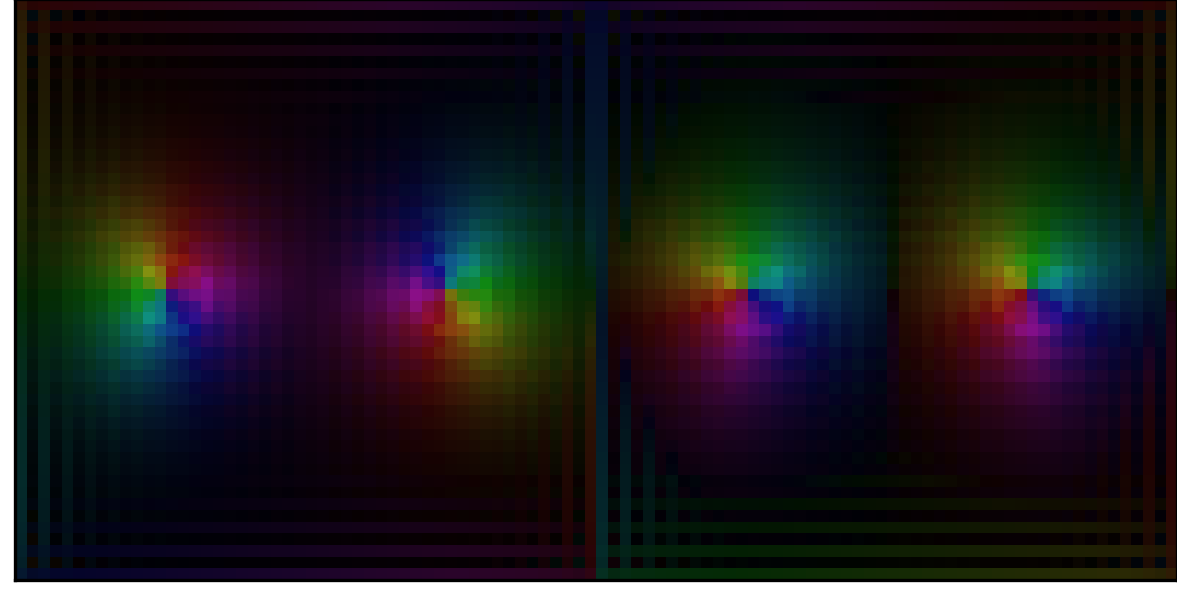
\includegraphics[width=\textwidth]{imgs/Mode_P_-4t_mu0.5_t0.25_D1.png}
    \caption{Complex plot of the $\vec{V}$ vector for $\mu_0 = 0.5, t = 0.25, \Delta = 1, radius = G/8$}
    \label{fig:Mode1}
\end{figure}
From \secref{sec:indChegeConjSym} we know that the $\vec{W}$ mode is just $\gamma \vec{V}^*$, so $\vec{W}$ plotted is just the complex conjugate of the $\vec{u}$ and  $\vec{v}$ plots swapped. We can verify this by calculating the error from \eqref{num:GenericErrorExpr} or by evaluating $|\vec{V}-\gamma \vec{W}^*|$ we typically get  values that are zero to numerical precision. In \figref{fig:Mode1} we can observe the two voritices and the phase winding of $2\pi$. In the $\vec{v}$ plot both modes have the same phase and chirality whereas in the $\vec{u}$ plot both vortices have opposing chirality and a $\pi$ phase difference. For these values of $\mu,t,\Delta$ in \figref{fig:Mode1} this plot becomes especially simple. For other parameters the statements above still are valid, but a more complex structure occurs.
The expectation value of the Density Change Operator $\left<\Delta \hat{n_{x,y}}\right>$ \eqref{bdg:Diffop} calculated as in \eqref{bdg:Expectationvalues} \eqref{bdg:DiffDens} of this mode is \figref{fig:Mode1Density} 
\begin{figure}[H]
    \centering
    \hspace*{2cm}
    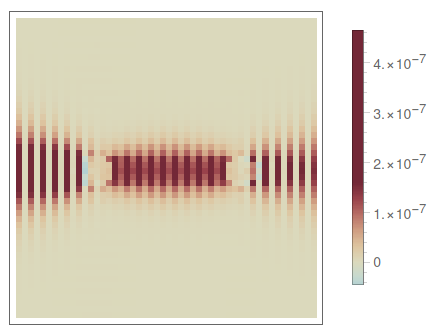
\includegraphics[width=0.7\textwidth]{imgs/DMode_P _-4t_mu0 .5_t0 .25_D1.png.png}
    \caption{$\left<\Delta \hat{n}_{x,y}\right>$ for the lowest energy $d^{\dag}$ operator at  $\mu_0 = 0.5, t = 0.25, \Delta = 1, radius = G/8$}
    \label{fig:Mode1Density}
\end{figure}
We observe that the change in electron-density is vanishingly small e.g. $\sum_{x,y}|\left<\Delta \hat{n}_{x,y}\right>| = 4.76734 \cdot 10^{-5}$ for \figref{fig:Mode1Density}, so the electron density of the the degenerate ground state is very similar.\\
We can also plot the Majorana modes in the same way. When we express the magnitude of the vector entries as in \figref{fig:MajMag}, we observe that they each Majorana mode operates only one of the two vortices. Here $\mathbf{\Gamma}_A$ operates on the right vortex and $\mathbf{\Gamma}_B$ on the left vortex.
\begin{figure}[H]
\centering
\begin{tabular}{cc}
     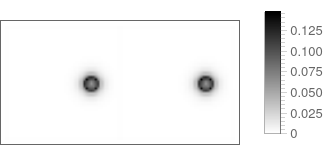
\includegraphics[width = 0.5\linewidth]{imgs/GA_P_-4t_mu0.5_t0.25_D1.png}&
     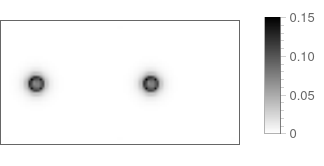
\includegraphics[width = 0.5\linewidth]{imgs/GB_P_-4t_mu0.5_t0.25_D1.png}\\
      $|\mathbf{\Gamma}_A|$&  $|\mathbf{\Gamma}_B|$
\end{tabular}
\caption{Plot of Majorana modes for $\mu_0 = 0.5, t = 0.25, \Delta = 1, radius = G/8$}
\label{fig:MajMag}
\end{figure}
\mypagebreak
A nice visualisation of the behaviour is provided by adding $\vec{u}+\vec{v}$.
This is due to the fact that when we take the $\vec{\Gamma}_A$ and $\vec{\Gamma}_B$ vectors and the fact that they are invariant under the induced charge conjugation symmetry $\mathcal{C}$. We can define:
$$
\vec{\Gamma_A} = 
\left(
\begin{array}{c}
     \vec{u}+\vec{v}^*  \\
     \hline
     \vec{v}+\vec{u}^* 
\end{array}\right)
= 
\left(
\begin{array}{c}
     \boldsymbol\alpha  \\
     \hline
     \boldsymbol\alpha^* 
\end{array}\right) 
$$$$
\vec{\Gamma_B} = -i
\left(
\begin{array}{c}
     \vec{u}-\vec{v}^*  \\
     \hline
     \vec{v}-\vec{u}^* 
\end{array}\right)
= 
\left(
\begin{array}{c}
     \boldsymbol\beta  \\
     \hline
     \boldsymbol\beta^* 
\end{array}\right) 
$$
Then it is
$$
\vec{u} = \frac{1}{2} (\boldsymbol\alpha + i \boldsymbol\beta ) \text{ and } \vec{v} =\frac{1}{2} (\boldsymbol\alpha^* + i \boldsymbol\beta^*)
$$
$$
\vec{u}+\vec{v}  = \frac{1}{2} (\boldsymbol\alpha + i \boldsymbol\beta + \boldsymbol\alpha^*  +i \boldsymbol\beta^*)
= \Re{\boldsymbol\alpha}+ i \Re{\boldsymbol\beta}
$$
As both modes have a $2\pi$ phase-winding, there is always a real part. Further, a phase becomes a rotation in the $\vec{u}+\vec{v}$ picture. We can differentiate between the A and B modes by colour and see the phase as a rotation.\\

\begin{figure}[H]
    \centering
    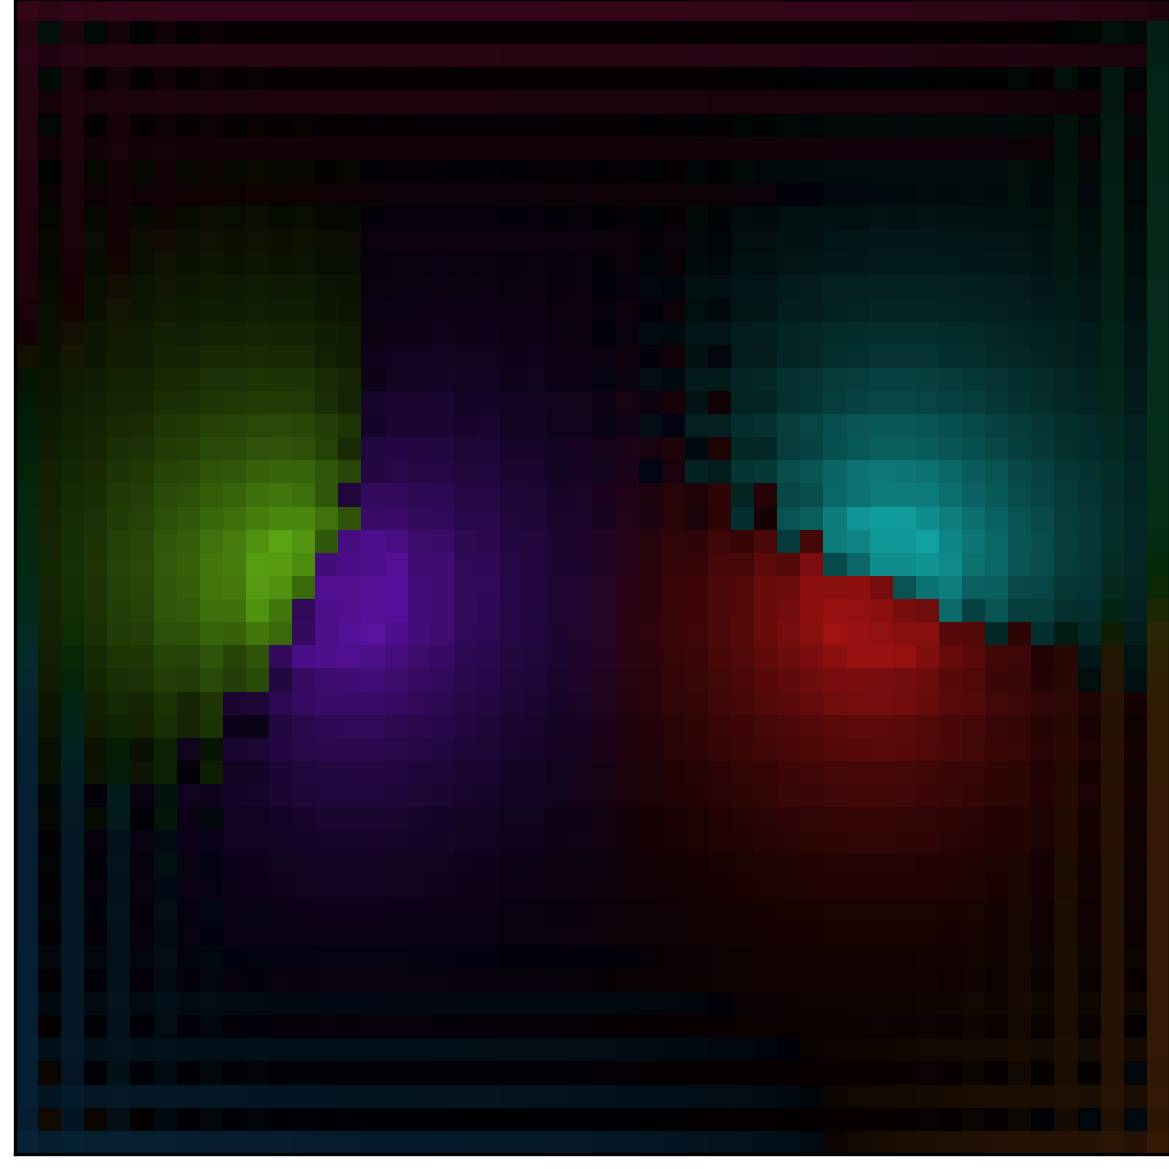
\includegraphics[width= 0.7\textwidth]{imgs/2D_Modex+y0.png}
    \caption{$\vec{u}+\vec{v}$ Plot for the $\vec{V}$ vector for $\mu_0 = 0.5, t = 0.25, \Delta = 1, radius = G/8$}
    \label{ilmig:UV}
\end{figure}
\mypagebreak
We can observe the energy-splitting of the edge mode in dependence to the vortex radius.
We use a larger  $80 \times 80$ grid for better resolution. As before we choose $t=\frac{1}{4}, \Delta = 1, \mu = \frac{1}{2}$
\begin{figure}[H]
    \centering
    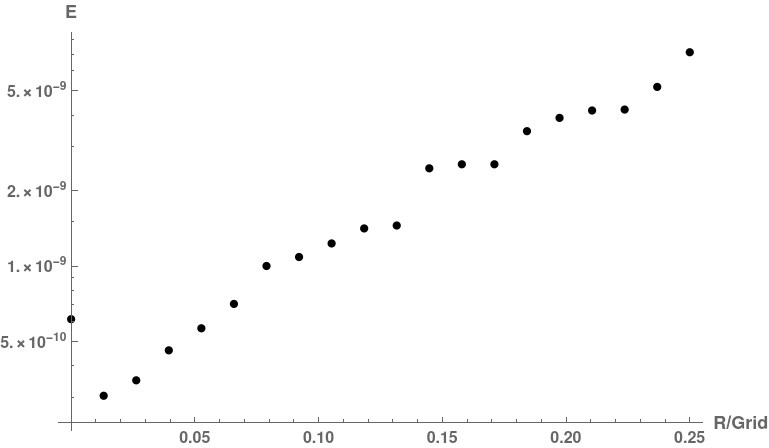
\includegraphics[width= 0.6 \textwidth]{imgs/R_E_Split.png}
    \caption{Logarithmic plot of lowest edge state energy for with varying vortex radius $t=\frac{1}{4}, \Delta = 1, \mu = \frac{1}{2}$}
    \label{fig:R_E_Split}
\end{figure}
We observe an exponential energy-splitting. When the radius is smaller than a single site the energy increases again. However, because  $\mu(r)$ is discrete values smaller, than 0.5 are unreasonable. We can also observe energy splitting as a function of the distance between vortices.
\begin{figure}[H]
    \centering
    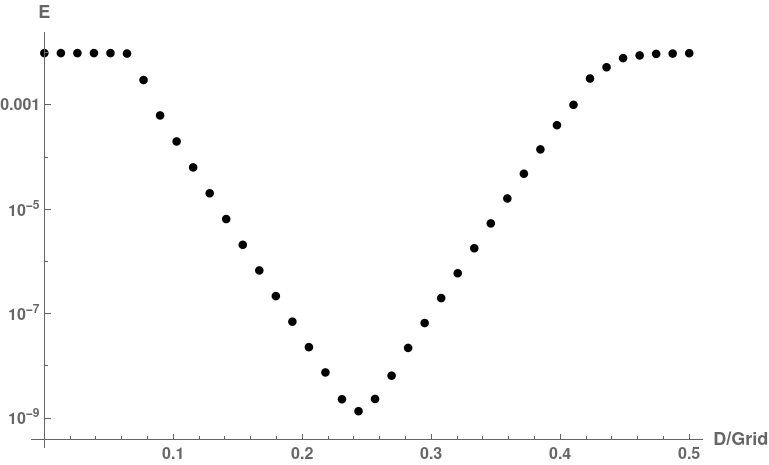
\includegraphics[width= 0.6 \textwidth]{imgs/D_E_Split.png}
    \caption{Logarithmic plot of lowest edge state energy for varying vortex to vortex distance D $t=\frac{1}{4}, \Delta = 1, \mu = \frac{1}{2}, R = G/8$}
    \label{fig:D_E_Split}
\end{figure}
The energy splitting depends on both the vortex-to-vortex distance and the vortex boundary distance. When the vortices touch each other or the boundary, the gap remains constant. The energy-splitting as a function of vortex-to-vortex distance is much stronger than the energy-splitting of the radius with about  6 orders of magnitude compared to one order of magnitude for the radius.
We once again observe an exponential energy-splitting.
\mypagebreak
\subsection{Adiabatic Time Evolution}
We can now look at the time evolution up to dynamic phase when a small energy splitting is present. We visualise the process by plotting the $\vec{u}+\vec{v}$ for the initial state $\theta =0^\circ$ , the intermediary state $\theta = 90^\circ$ and final state $\theta = 180^\circ$. The orientation of rotation is shown with white arrows on the intermediary state and the identical vortices are connected by coloured dotted lines in \figref{fig:Film_exchange}.
\begin{figure}[H]
\centering
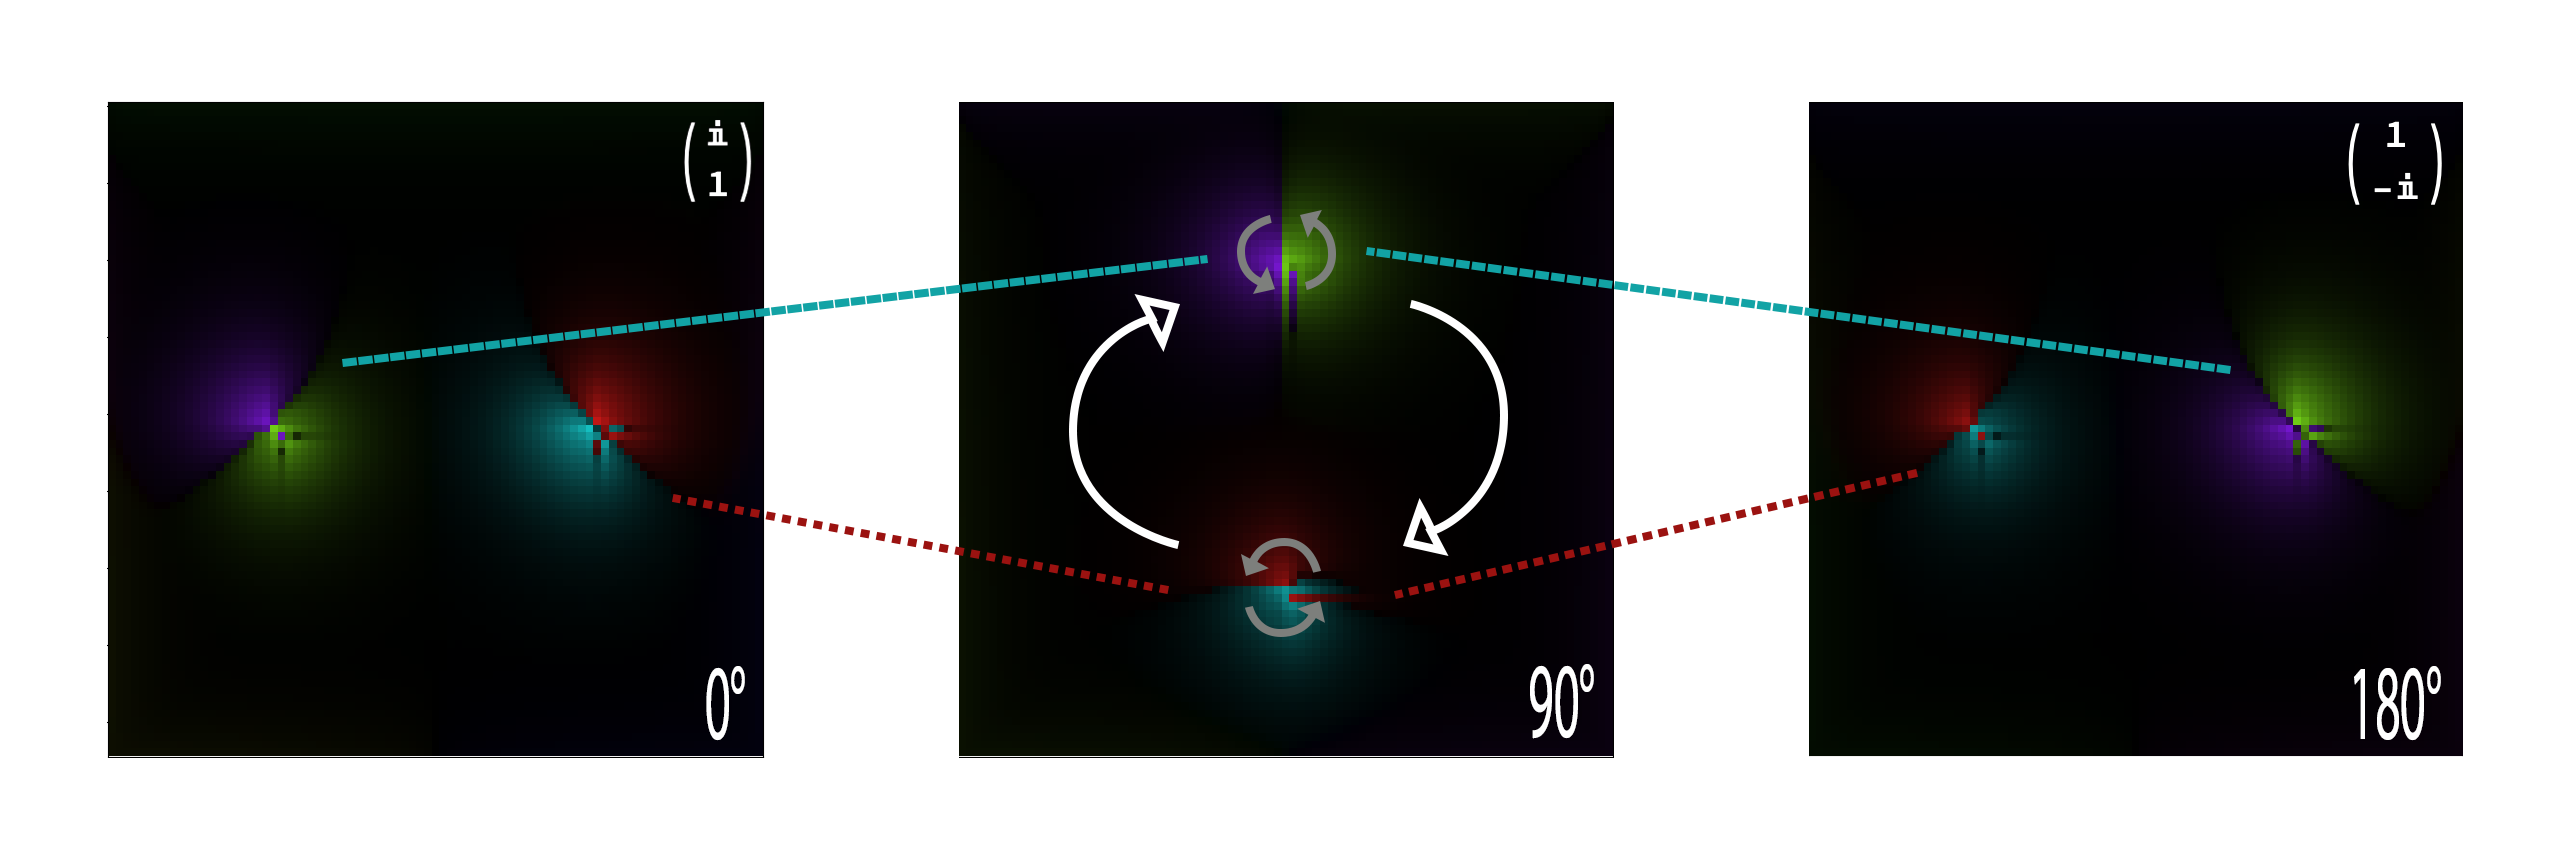
\includegraphics[width=\linewidth]{imgs/Test_Filmstrip_3.png}
  \caption{Complex plot $ u_{x,y}+v_{x,y} $ of  $\gamma_A$ during exchange}
  \label{fig:Film_exchange}
\end{figure}
We find that the vortices do exchange as predicted. We also observe a global $\pi/2$ phase. However, this phase is necessary to map the $\gamma_A$ mode to the $\gamma_B$ mode. Indeed, we observe that the $\gamma_A$ mode initially on the right in red ($1$) and cyan ($-1$) now sits at the position of $\gamma_B$. Further more the red region now sits where the purple ($i$) region of $\gamma_B$ used to be indicated by the red dotted line. However for $\gamma_B$ the case is different, as the purple region of $\gamma_B$ now sits where the cyan (-1) region of $\gamma_A$ used to be indicated by the dotted cyan line. Indicating a minus sign in the exchange. Surprisingly this recovers the complete exchange statistic from \secref{sec:ExhcangeStat} for $\sigma_1^{-1}$.
$$
T(\sigma_1^{-1}) = 
\left(
\begin{array}{cc}
    0 & -1 \\
    1 & 0
\end{array}
\right)
$$
 However, a phase of $\pi$ will swap the exchange statistic $\sigma_1^{-1} \leftrightarrow \sigma_1$ just as doing the exchange anti clockwise.\\
 
As demonstrated in equation \eqref{eq:ExPeriodicity} , we can attain four different states with this exchange. These states are shown in  \figref{fig:NAExchange_Map}:
\begin{figure}[H]
\centering
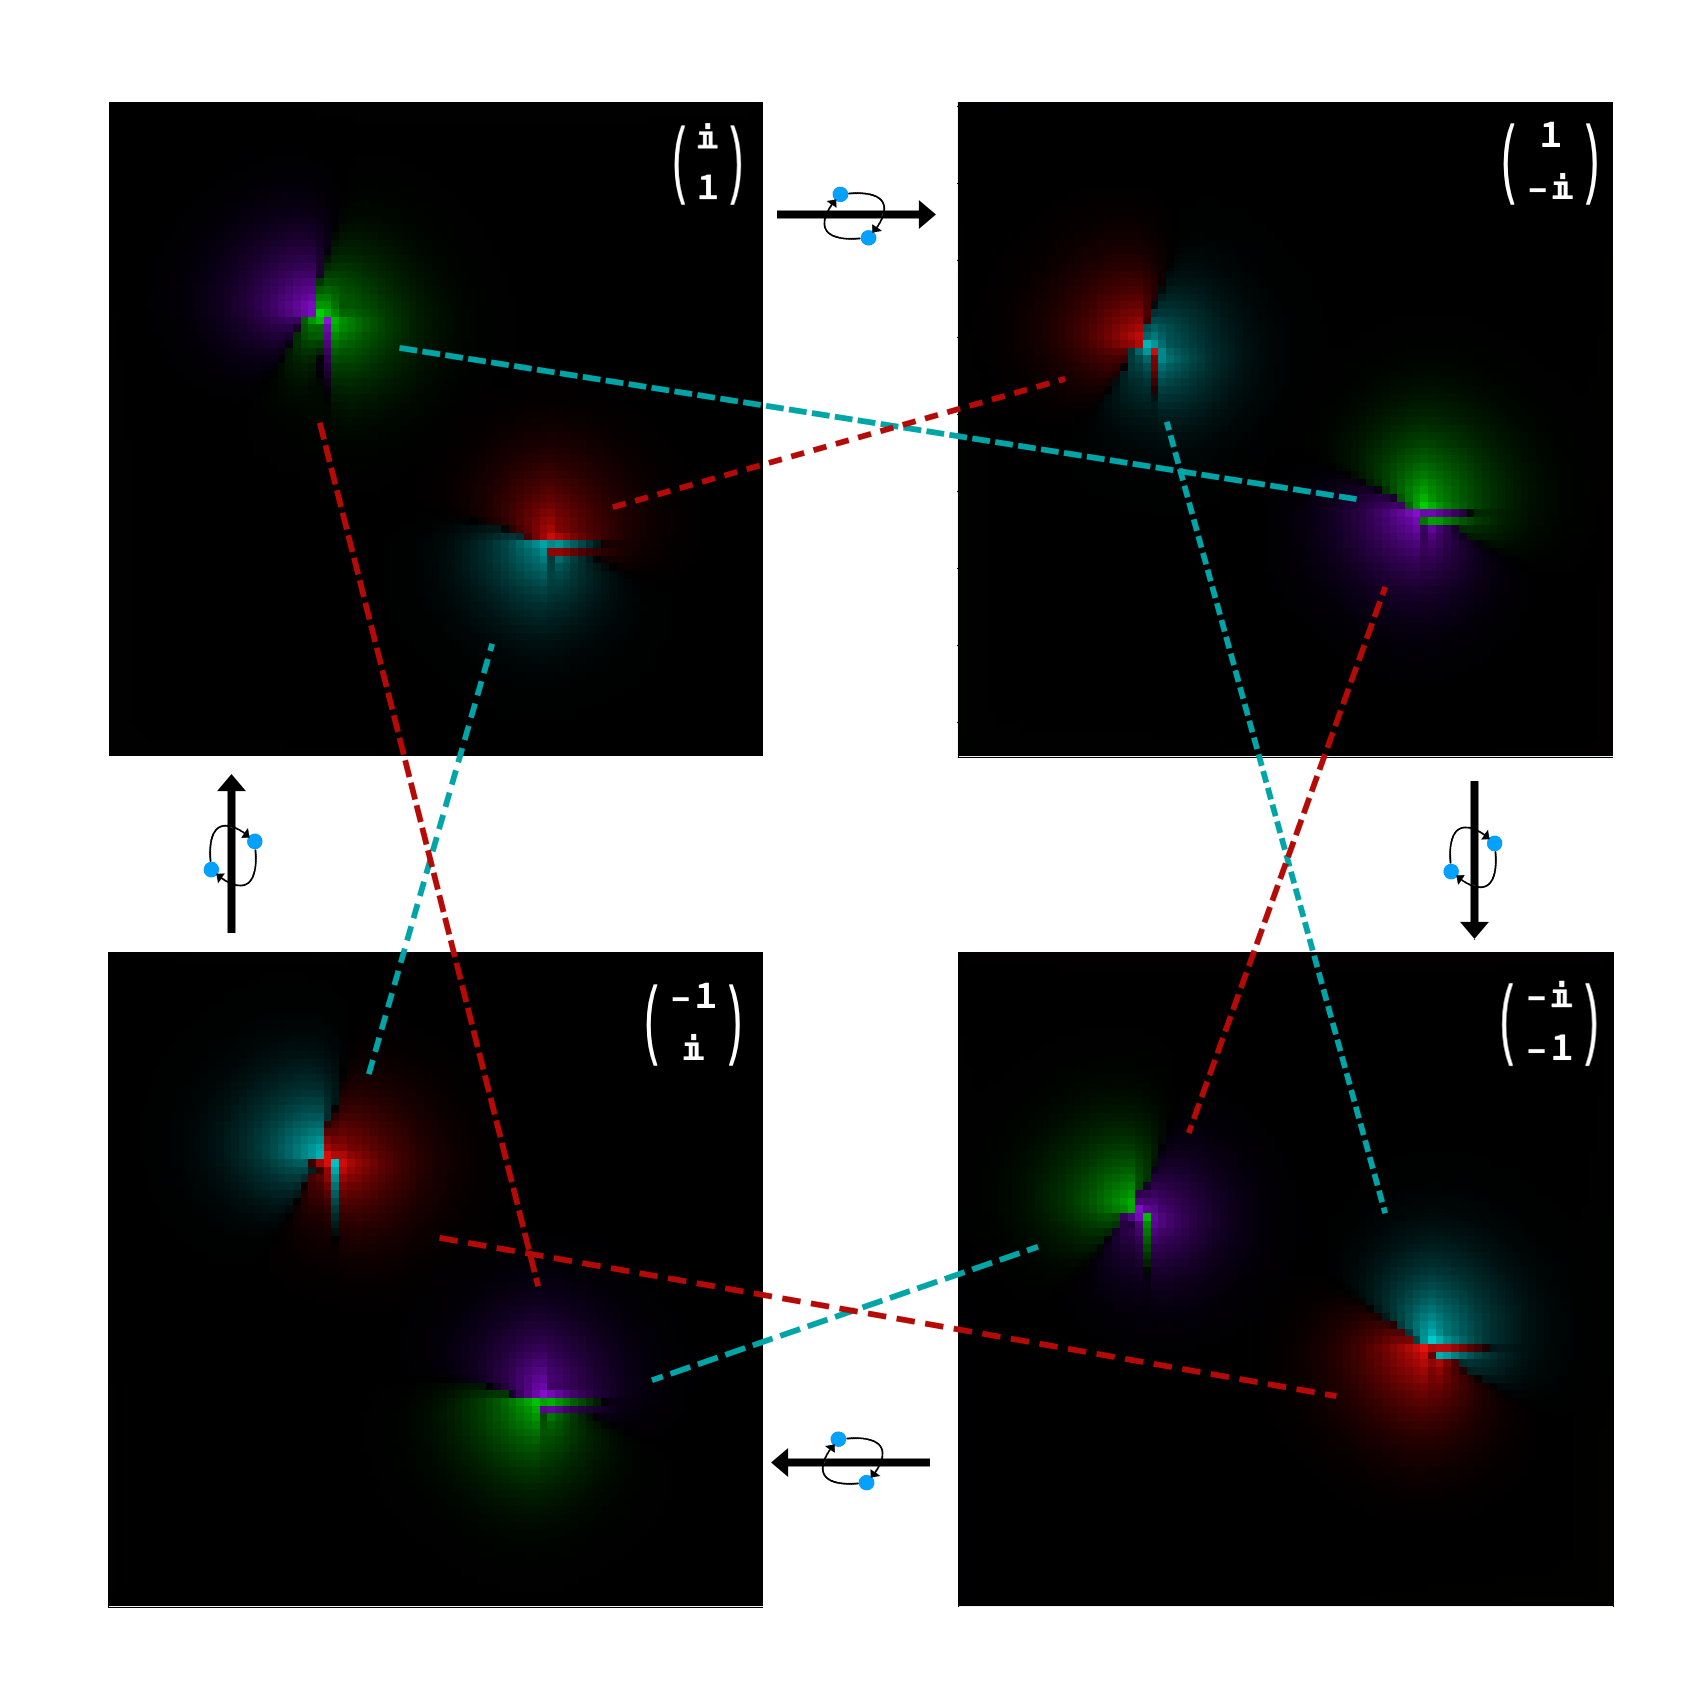
\includegraphics[width=0.9\linewidth]{imgs/Non-Abelian-Exchange_new.png}
  \caption{Complex plots $ u_{x,y}+v_{x,y}$ mapping all four different states.}
  \label{fig:NAExchange_Map}
\end{figure}
Moving clockwise through the 4 images, the vortices are exchanged clockwise between every image. Or counter-clockwise when moving counter-clockwise though the 4 pictures. The identical vortices are connected by dotted lines, whose colour indicates the sign the majorana mode at the vortex has picked up by the exchange. The vector in the top left indicates the sign of the modes in the picture, i denoting the $\gamma_B$ mode.
Further images of the exchange including plots of $\vec{u}+ \vec{v}$ \figref{fig:AdTevl+} $\vec{u}$ and $ \vec{v}$ \figref{fig:AdTevl} separately can be found in \secref{sec:AppendixA}
\mypagebreak
\subsection{Non-Adiabatic Time Evolution}
We now observe the exchange of Majorana modes outside the adiabatic regime. 
\subsubsection{Two  Vortices}
From \secref{sec:Propagator} we have an expression for the propagator $K(l',l,t)$ at $T=0$ in terms of the the scalar product for operators defined in \eqref{BdG:Prop=Scal}  when the operators are in reverse normal order or the expression is zero. 
We compute the time evolution of the creation operator $d^{\dag}(t) = U(t)d^{\dag}U^{\dag}(t)$.
We evaluate the propagator for the edge mode creator and annihilator operators for $d,d^{\dag}$ $\left<d| d^{\dag}(-\pi/\omega)\right>$ and $\left< d^{\dag}(-\pi/\omega)|d^{\dag}\right>$in dependence of $\omega$ .
We compare the result with the adiabatic case. We assume a vanishing energy-splitting and the exchange statistic \eqref{eq:2VortExchange} from \secref{sec:ExhcangeStat} as our time evolution. With $d^{\dag}\ket{0} = \ket{1}$
 we expect:
$$
\left<d d^{\dag}(-\pi/\omega)\right> = \bra{1} \tau(\sigma) d^{\dag}\tau(\sigma^{-1})\ket{0}
= \bra{1} \tau(\sigma) d^\dag e^{- \frac{i \pi}{4}}\ket{0} = e^{\frac{i \pi}{4}} \bra{1} \tau(\sigma) \ket{1} = e^{- \frac{i \pi}{2}}
$$
$$
\left< d^{\dag}(-\pi/\omega)d^{\dag}\right>  
= \bra{0} \tau(\sigma) d^\dag \tau(\sigma^{-1})\ket{1} = e^{-\frac{i \pi}{4}} \bra{1} \tau(\sigma) d^{\dag} \ket{1} = 0
$$
For the diabatic case, we expect $\left<dd^{\dag}\right> = 1 - \left<\hat{n}\right> = 1$ and $\left<d^{\dag}d^{\dag}\right> = 0$.
The magnitude squared of the propagators $\left<d| d^{\dag}(-\pi/\omega)\right>$ and $\left< d^{\dag}(-\pi/\omega)|d^{\dag}\right>$ corresponds to the fidelity. We further plot the inner product of the time evolved creation operator to the Majorana creation and annihilation operators at $t=0$ $\left<\gamma_A| d^{\dag}(-\pi/\omega)\right>,\left<\gamma_B| d^{\dag}(-\pi/\omega)\right>,\left< d^{\dag}(-\pi/\omega)|\gamma_A\right>$ and $\left< d^{\dag}(-\pi/\omega)|\gamma_B\right>$.
\mypagebreak
\begin{figure}[H]
    \centering
    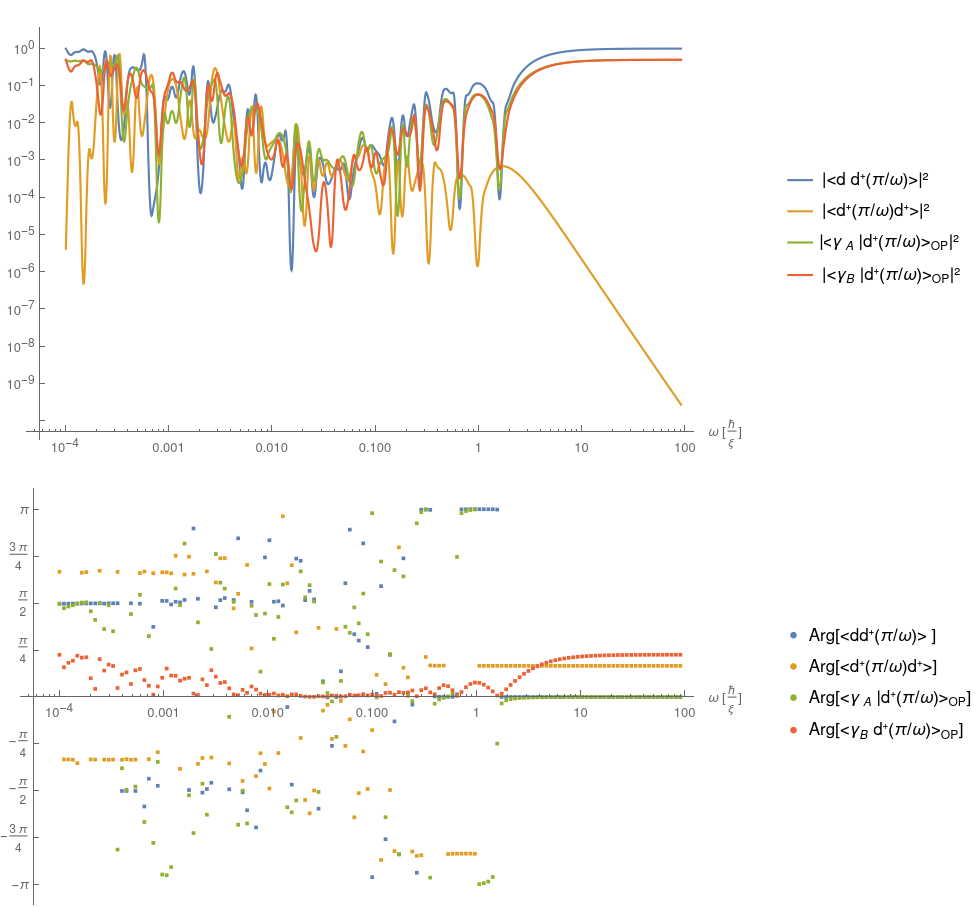
\includegraphics[width=\textwidth]{imgs/2VortSmall.png}
    \caption{Time evolution of the exchange of two Gaussian vortices $\mu = 1, \Delta = 1, t = -\frac{2}{3}, R = \frac{1}{35}$}
    \label{fig:2VortExchange}
\end{figure}
We can observe that for $\omega >> 1$, we are in the diadiabatic regime. We can also observe the beginning of the adiabatic regime at $\omega < 10^{-4}$. In the regime between we observe oscillatory behaviour with sharp points where $\left<d d^{\dag}(-\pi/\omega)\right>$ becomes large and $\left<d^{\dag}(-\pi/\omega)d^{\dag}\right>$ small. 
We can also plot the fidelity in dependence to the radius.
\begin{figure}[H]
    \centering
    \begin{tabular}{c}
         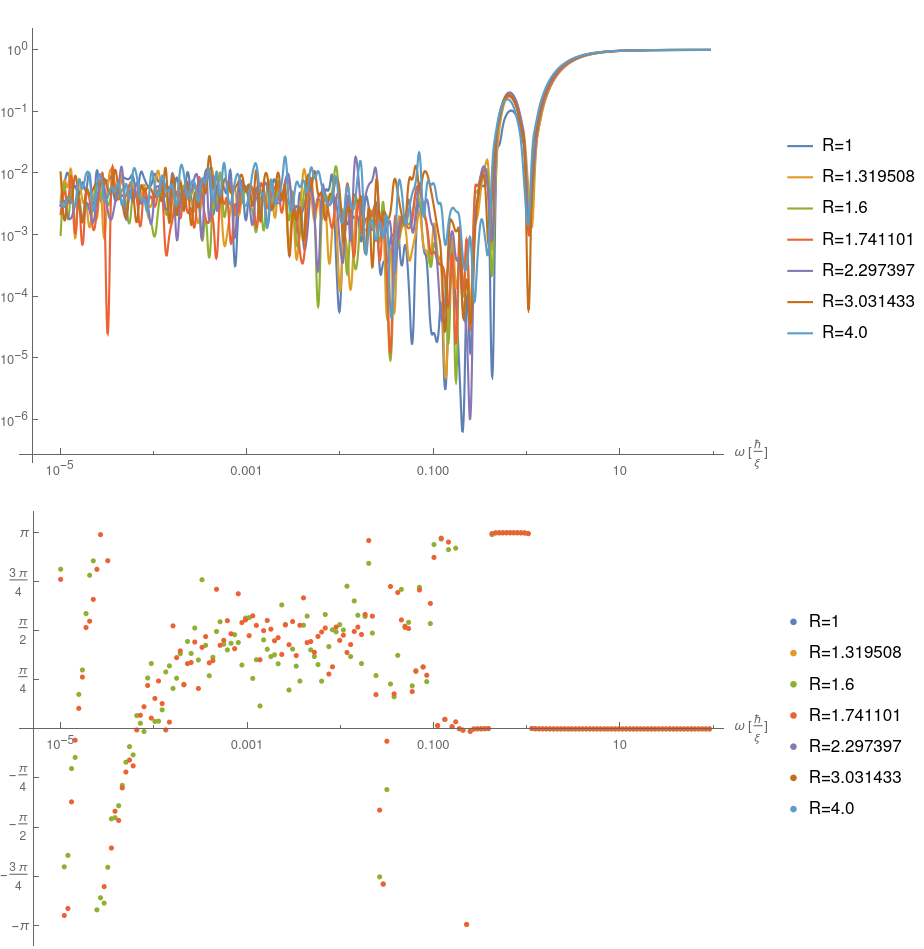
\includegraphics[width=\textwidth]{imgs/Fidellity_Rad.png}\\
    \end{tabular}
    \caption{Comparison of the fidelity $|\left<d d^{\dag}(-\pi/\omega)\right>|^2$ for the exchange of two discrete vortices $\mu = 0.5, \Delta = 1, t = \frac{1}{2}$ and distance $D=9$ with a $-4t$ shift and different vortex radii $R$}
    \label{fig:R_Fid_Phase}
\end{figure}
\begin{figure}[H]
    \centering
    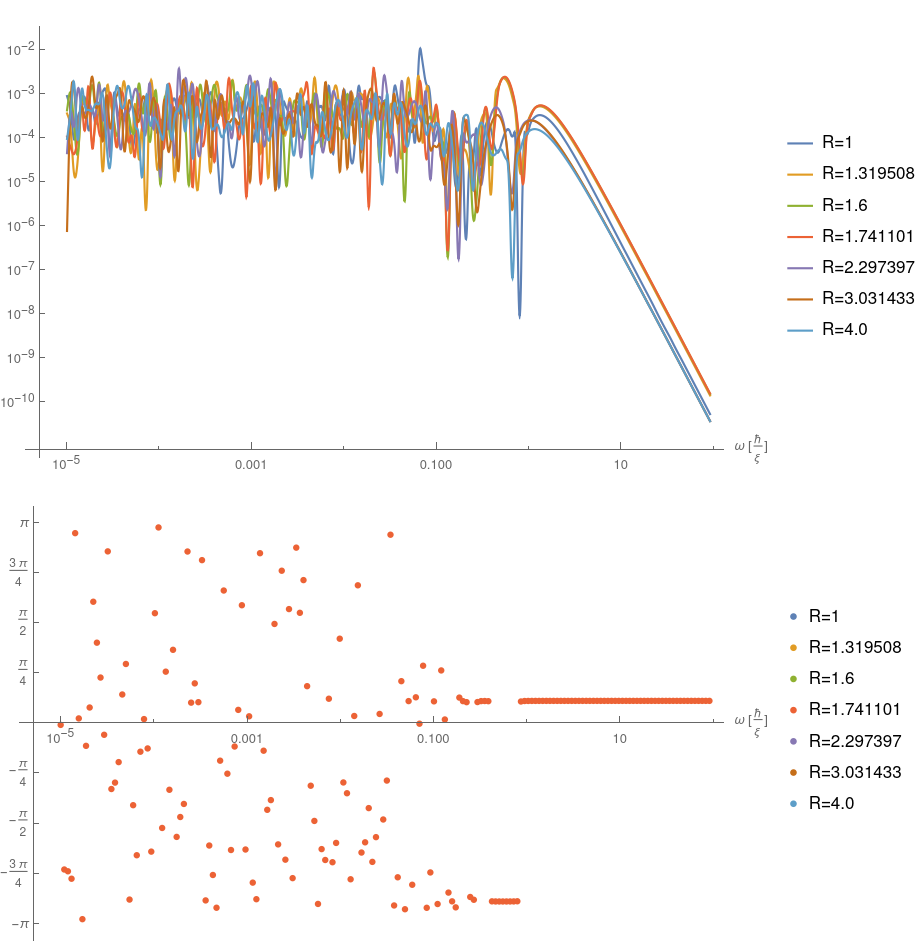
\includegraphics[width=\textwidth]{imgs/Fidellity_Rad2.png}
    \caption{Comparison of the fidelity $|\left<(-\pi/\omega)d^{\dag}\right>|^2$ for the exchange of two discrete vortices $\mu = 1, \Delta = 1, t = \frac{1}{2}$ and distance $D=9$ with a $-4t$ shift and different vortex radii $R$}
    \label{fig:R_Fid_Phase2}
\end{figure}
In both \figref{fig:R_Fid_Phase} and \figref{fig:R_Fid_Phase2}, we demonstrate that the increasing radius shifts the adiabatic regime to longer and diadiabatic regime to shorter exchange times.
We can also plot the fidelity in dependence to the distance $D$.
\begin{figure}[H]
    \centering
    \begin{tabular}{c}
         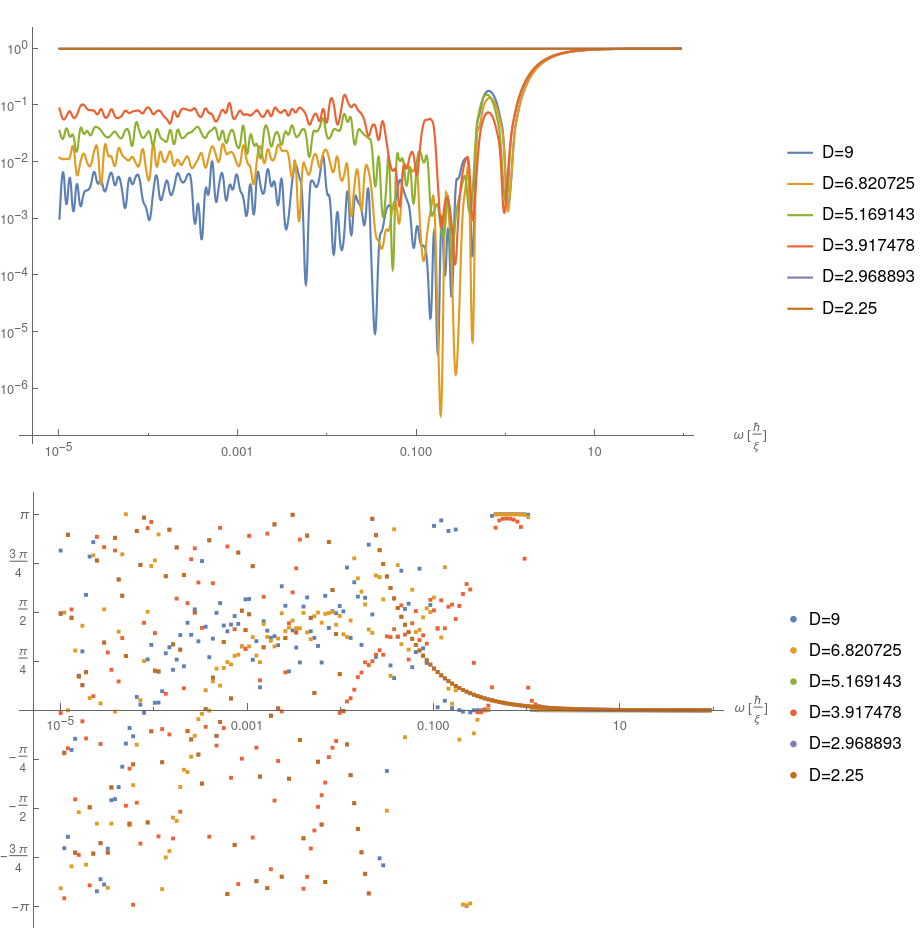
\includegraphics[width=\textwidth]{imgs/Fidellity_Dist.png}\\
    \end{tabular}
    \caption{Comparison of the fidelity $|\left<d d^{\dag}(-\pi/\omega)\right>|^2$ for the exchange of two discrete vortices $\mu = 0.5, \Delta = 1, t = \frac{1}{2}$ and radius $R=1.6$ with a $-4t$ shift and different vortex Distances $D$}
    \label{fig:D_Fid_Phase}
\end{figure}
We observe that for a distance $D$ smaller, than two times the radius $D<2*R = 3.2$ no exchange occurs, as the vortices merge into a single vortex.
\begin{figure}[H]
    \centering
    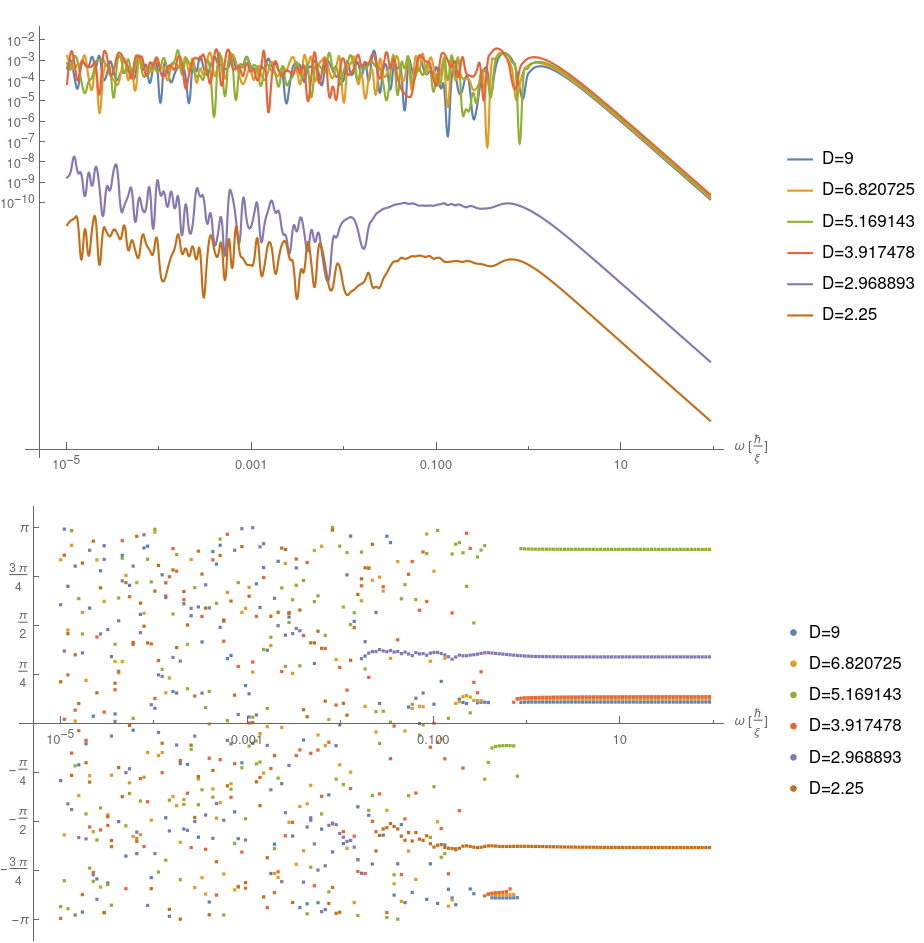
\includegraphics[width=\textwidth]{imgs/Fidellity_Dist2.png}
    \caption{Comparison of the fidelity $|\left<(-\pi/\omega)d^{\dag}\right>|^2$ for the exchange of two discrete vortices $\mu = 1, \Delta = 1, t = \frac{1}{2}$ and radius $R=1.6$ with a $-4t$ shift and different vortex Distances $D$}
    \label{fig:D_Fid_Phase2}
\end{figure}
In both \figref{fig:D_Fid_Phase} and \figref{fig:D_Fid_Phase2}, we demonstrate that the decreasing Distance decreases the Fidelity. The effect is stronger for the vortex distance than for the vortex radius, As is expected from the calculations of the Energy shift.
\pagebreak 
\subsubsection{Four Vortices}
Analogous to the two vortices, we evaluate the propagator in the four vortex case. Here, the adiabatic time evolution of zero-energy edge states can behave in one of three ways. The three ways in  \secref{sec:ExhcangeStat}  $\tau(\sigma_1), \tau(\sigma_2), \tau(\sigma_2)$ correspond to the three generators of the Braid Group $\mathcal{B}_4$. $\sigma_1$ and $\sigma_3$ correspond to an exchange of Majorana modes from the same edge state and behave analogously to the two vortex case.
The $\sigma_2$ exchange corresponds to an exchange of two Majorana modes from different edge modes.
We evaluate $\left<d_1 d_1^{\dag}(-\pi/\omega)\right>$, $\left<d_2 d_1^{\dag}(-\pi/\omega)\right>$ $\left<d_1^{\dag}(-\pi/\omega) d_1^{\dag}\right>$, $\left<d_1^{\dag}(-\pi/\omega) d_2^{\dag}\right>$. For the diabatic case we expect all Propagators to be zero except $\left<d_1 d_1^{\dag}(-\pi/\omega)\right>=1$and expect for the adiabatic case:
$$
\left<d_1 d_1^{\dag}(-\pi/\omega)\right> = \underbrace{\bra{0} d_1}_{= \bra{1,0}} \tau(\sigma_3) d_1^{\dag}\tau(\sigma_3)^{\dag}\ket{0}
= \bra{1,0} \tau(\sigma_3) d_1^\dag \frac{1}{\sqrt{2}}(\ket{0}+i \ket{1,1})
$$
$$ =  \frac{1}{\sqrt{2}}\bra{1,0} \tau(\sigma_3) \ket{1,0} = \frac{1}{2}\bra{1,0} (\ket{1,0}-i\ket{0,1}) = \frac{1}{2}
$$
$$
\left<d_2 d_1^{\dag}(-\pi/\omega)\right> = \bra{0,1} \tau(\sigma_3) d_1^{\dag}\tau(\sigma_3)^{\dag}\ket{0}
= \bra{0,1} \tau(\sigma_3) d_1^\dag \frac{1}{\sqrt{2}}(\ket{0}+i \ket{1,1}) =
$$
$$
\frac{1}{\sqrt{2}}\bra{0,1} \tau(\sigma_3) \ket{1,0} = \frac{1}{2}\bra{0,1} (\ket{1,0}-i\ket{0,1}) = -\frac{i}{2}
$$
$$
\left<d_1^{\dag}(-\pi/\omega) d_1^{\dag}\right> = \bra{0}  \tau(\sigma_3) d_1^{\dag} \tau(\sigma_3)^{\dag}\ket{1,0}
= \bra{0}  \tau(\sigma_3) d_1^{\dag} \frac{1}{\sqrt{2}} (\ket{1,0} + i\ket{0,1})
$$
$$ = \frac{1}{\sqrt{2}} \bra{0}  \tau(\sigma_3) d_1^{\dag}  (\ket{1,0} + i\ket{0,1}) =  \frac{i}{\sqrt{2}} \bra{0}  \tau(\sigma_3)  \ket{1,1}) = \frac{i}{2} \bra{0} (\ket{1,1}-i \ket{0}) = \frac{1}{2}
$$
$$
\left<d_1^{\dag}(-\pi/\omega) d_2^{\dag}\right> = \bra{0}  \tau(\sigma_3) d_1^{\dag} \tau(\sigma_3)^{\dag} \ket{0,1} = \bra{0}  \tau(\sigma_3) d_1^{\dag} \frac{1}{\sqrt{2}}(\ket{0,1} + i \ket{1,0})
$$
$$
 = \frac{1}{\sqrt{2}} \bra{0}  \tau(\sigma_3) \ket{1,1} = \frac{1}{2} \bra{0} (\ket{1,1} - i \ket{0}) = \frac{-i}{2}
$$
 \mypagebreak
 
\begin{figure}[H]
\begin{tabular}{c}
     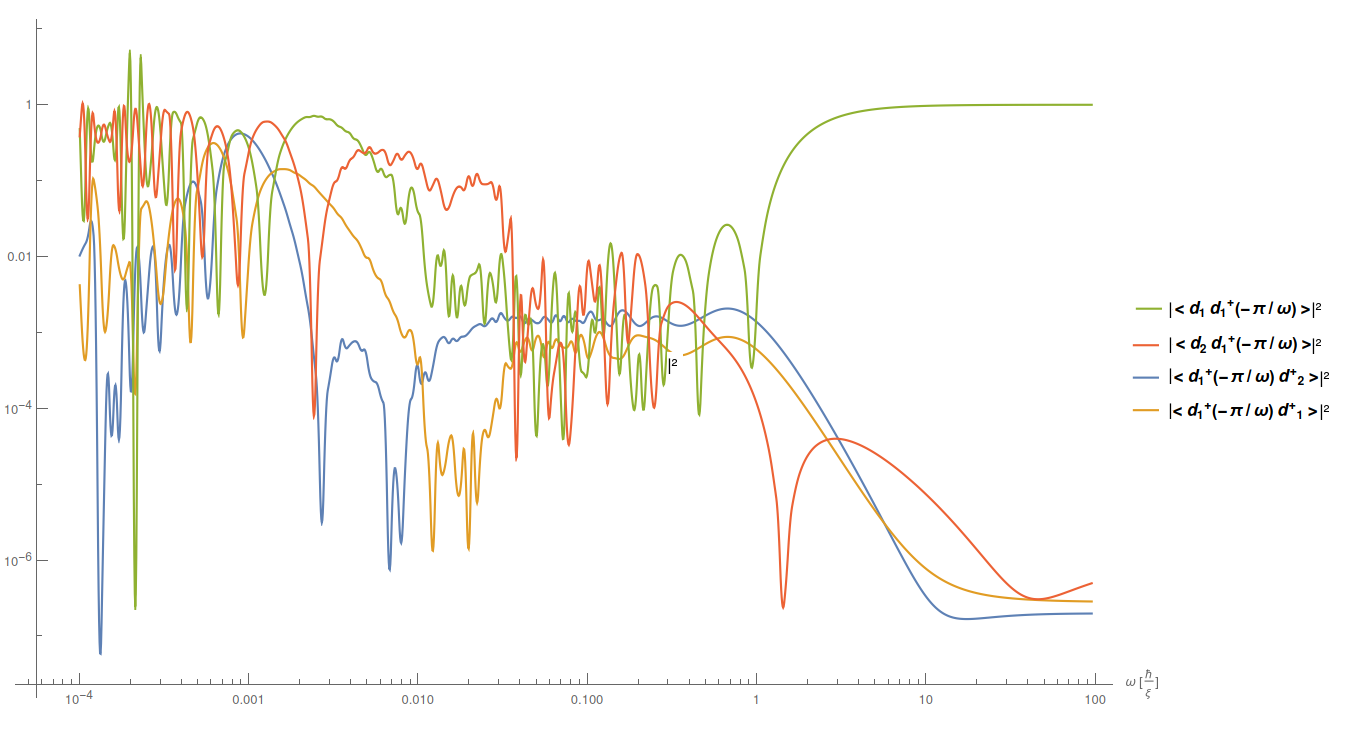
\includegraphics[width=\textwidth, left]{imgs/4VortFid.png} \\
    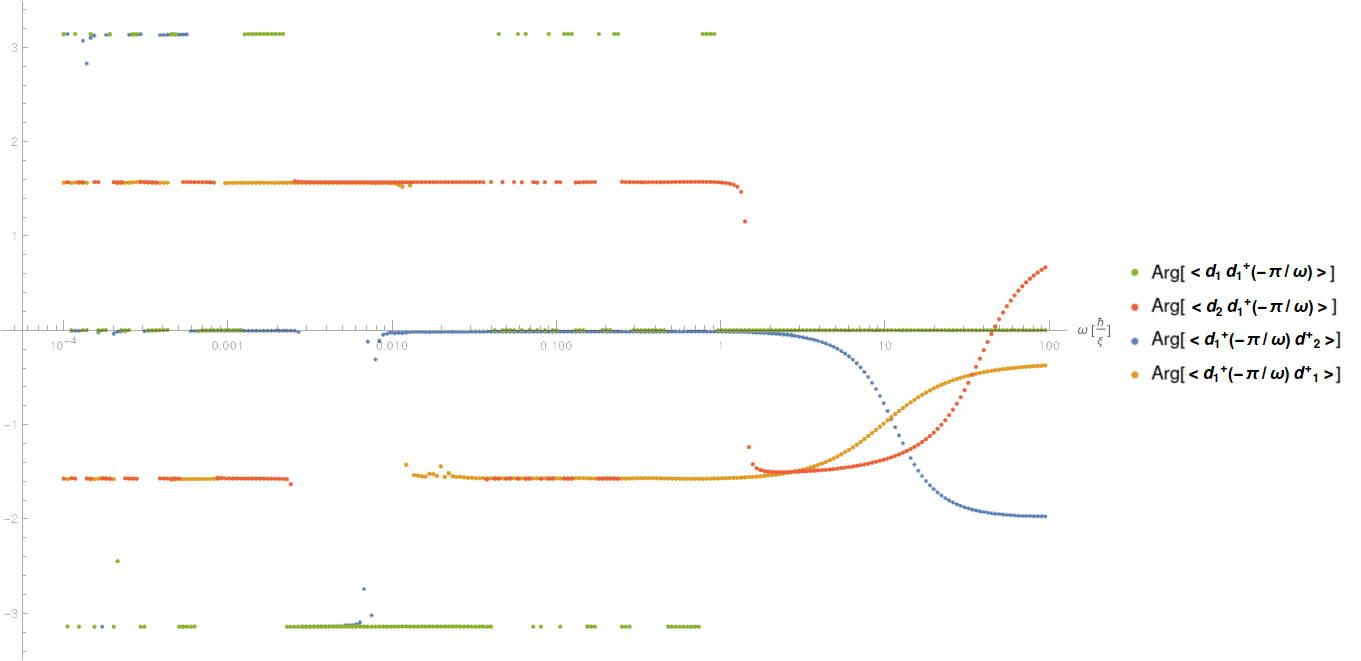
\includegraphics[width=0.8\textwidth,left]{imgs/4VortPhase.png}
\end{tabular}
    \caption{Exchange of $\tau(\sigma_2)$ of two Gaussian vortices $\mu = 1, \Delta = 1, t = -\frac{2}{3}, R = \frac{1}{35}$}
    \label{fig:sigma_1}
\end{figure}
\end{document}